\documentclass[12pt]{ctexart}
\usepackage[utf8]{inputenc}
\usepackage{geometry}
\geometry{left=1in,top=2.25in}
% \setlength{\parindent}{1em}
\setlength{\parskip}{1em}
\usepackage{xeCJK}    % 加载 xeCJK 宏包以支持中文
\usepackage{graphicx}
\usepackage{subfigure}
\usepackage{booktabs} % 导入booktabs包,用于创建三线表格
\usepackage{multirow}
\usepackage{amsmath}
\usepackage{hyperref}
\usepackage{amsfonts}
\usepackage{indentfirst} % 加载 indentfirst 宏包以使首段缩进
\usepackage{enumitem}
\setlist[enumerate]{label=(\arabic*)}
\usepackage{titlesec}
% \titlespacing{\section}{0pt}{\parskip}{-\parskip}
% \titleformat{\section}[block]{\normalfont\Large\bfseries}{\thesection}{1em}{}[\hspace{\parindent}] % 设置每个section第一段不缩进
% 设置绿色的引用和链接
\hypersetup{
    colorlinks=true,
    citecolor=green,
    linkcolor=green,
    filecolor=magenta,      
    urlcolor=cyan,
}

% 在目录中恢复原来的颜色
\makeatletter
\AtBeginDocument{%
  \pretocmd{\tableofcontents}{\hypersetup{citecolor=black,linkcolor=black}}{}{}%
}
\makeatother

% 设置 tocdepth 为 2,目录仅显示到二级标题
\setcounter{tocdepth}{3}

\usepackage{tocloft}

% 设置目录条目的行间距
\setlength{\cftbeforesecskip}{2.5ex} % 这里的 1ex 是你可以调整的行间距



\title{
\Huge{\textbf{商业分析报告}}\\
\Large{\textbf{BUSNESS ANALYSIS REPORT}}\\
\vspace{8mm}
% 
\includegraphics[width=5cm]{Images/logo.png}\\
% \vspace{25mm}
}
\author{\textbf{Week 1} \\
\textbf{AUTHOR: 杨唯茜 Estella}\\
% \textbf{Student Number: 202119293}\\
% Supervisors: \\
}
\date{DATE.vr1: 2024/09/10 \\
      DATE.vr2: 2024/09/17}




\pagestyle{empty}

\begin{document}
\newgeometry{right=1in,left=1in,top=1.5in,bottom=0.75in}
\maketitle
\thispagestyle{empty} % 去页数标记

\vspace{5mm}





\newpage
\clearpage
\thispagestyle{empty}
\newgeometry{right=0.75in,left=0.75in,top=1in,bottom=1in}
\thispagestyle{empty} % 去页数标记
\begin{titlepage}
{
\clearpage
\thispagestyle{empty}
  % 在目录之前设置颜色
  \color{black}
  \tableofcontents
}
\end{titlepage}
\newpage


\pagestyle{plain} 

\clearpage % 插入空白页
\pagenumbering{arabic}

\section{电子商务行业宏观形式}
%%% 章节框架:不确定因素的普遍存在 - 其他人的解决方法 - 给出普适的模型

% 1.1节(已完成)
\subsection{全球电商市场规模与发展趋势}
\begin{quote}
    \textit{“互联网给了普通人前所未有的力量去与全球的消费者进行互动,这不仅仅是技术的进步,也是电子商务的一场革命。”} \\
    \raggedleft \textit{- Mark Zuckerberg}
\end{quote}

科技发展催生产业升级与改型。随着数字化时代的到来,零售不再局限于路沿小型商超,卖家与顾客甚至不需要见面就可以完成交易。自1991年起,互联网就被开始用作商业载体,1995年,第一本在Amazon线上交易的书被卖出,这是电子商务活动的“起源”,同年,eBay也推出了电商交易活动。三年后,PayPal线上支付系统被推出,这是一针刺激市场的催化剂,随即Alibaba、Google、Yahoo等就接连拓展了其电商交易业务。电子商务活动能大幅拓宽交易选择面、简化交易流程并加速资金涌动,电商市场随即应运而生,势如破竹,拓展了传统贸易模式的地理局限性,为各路投资者所爱,至此起,电商市场蓬勃发展,市场规模也稳步增大。根据Statista的预测\cite{1},2024年全球电商零售收入额将超6.3万亿美元,在总零售收入额中占比20.1\%。

\begin{figure}[htbp!]
    \centering
    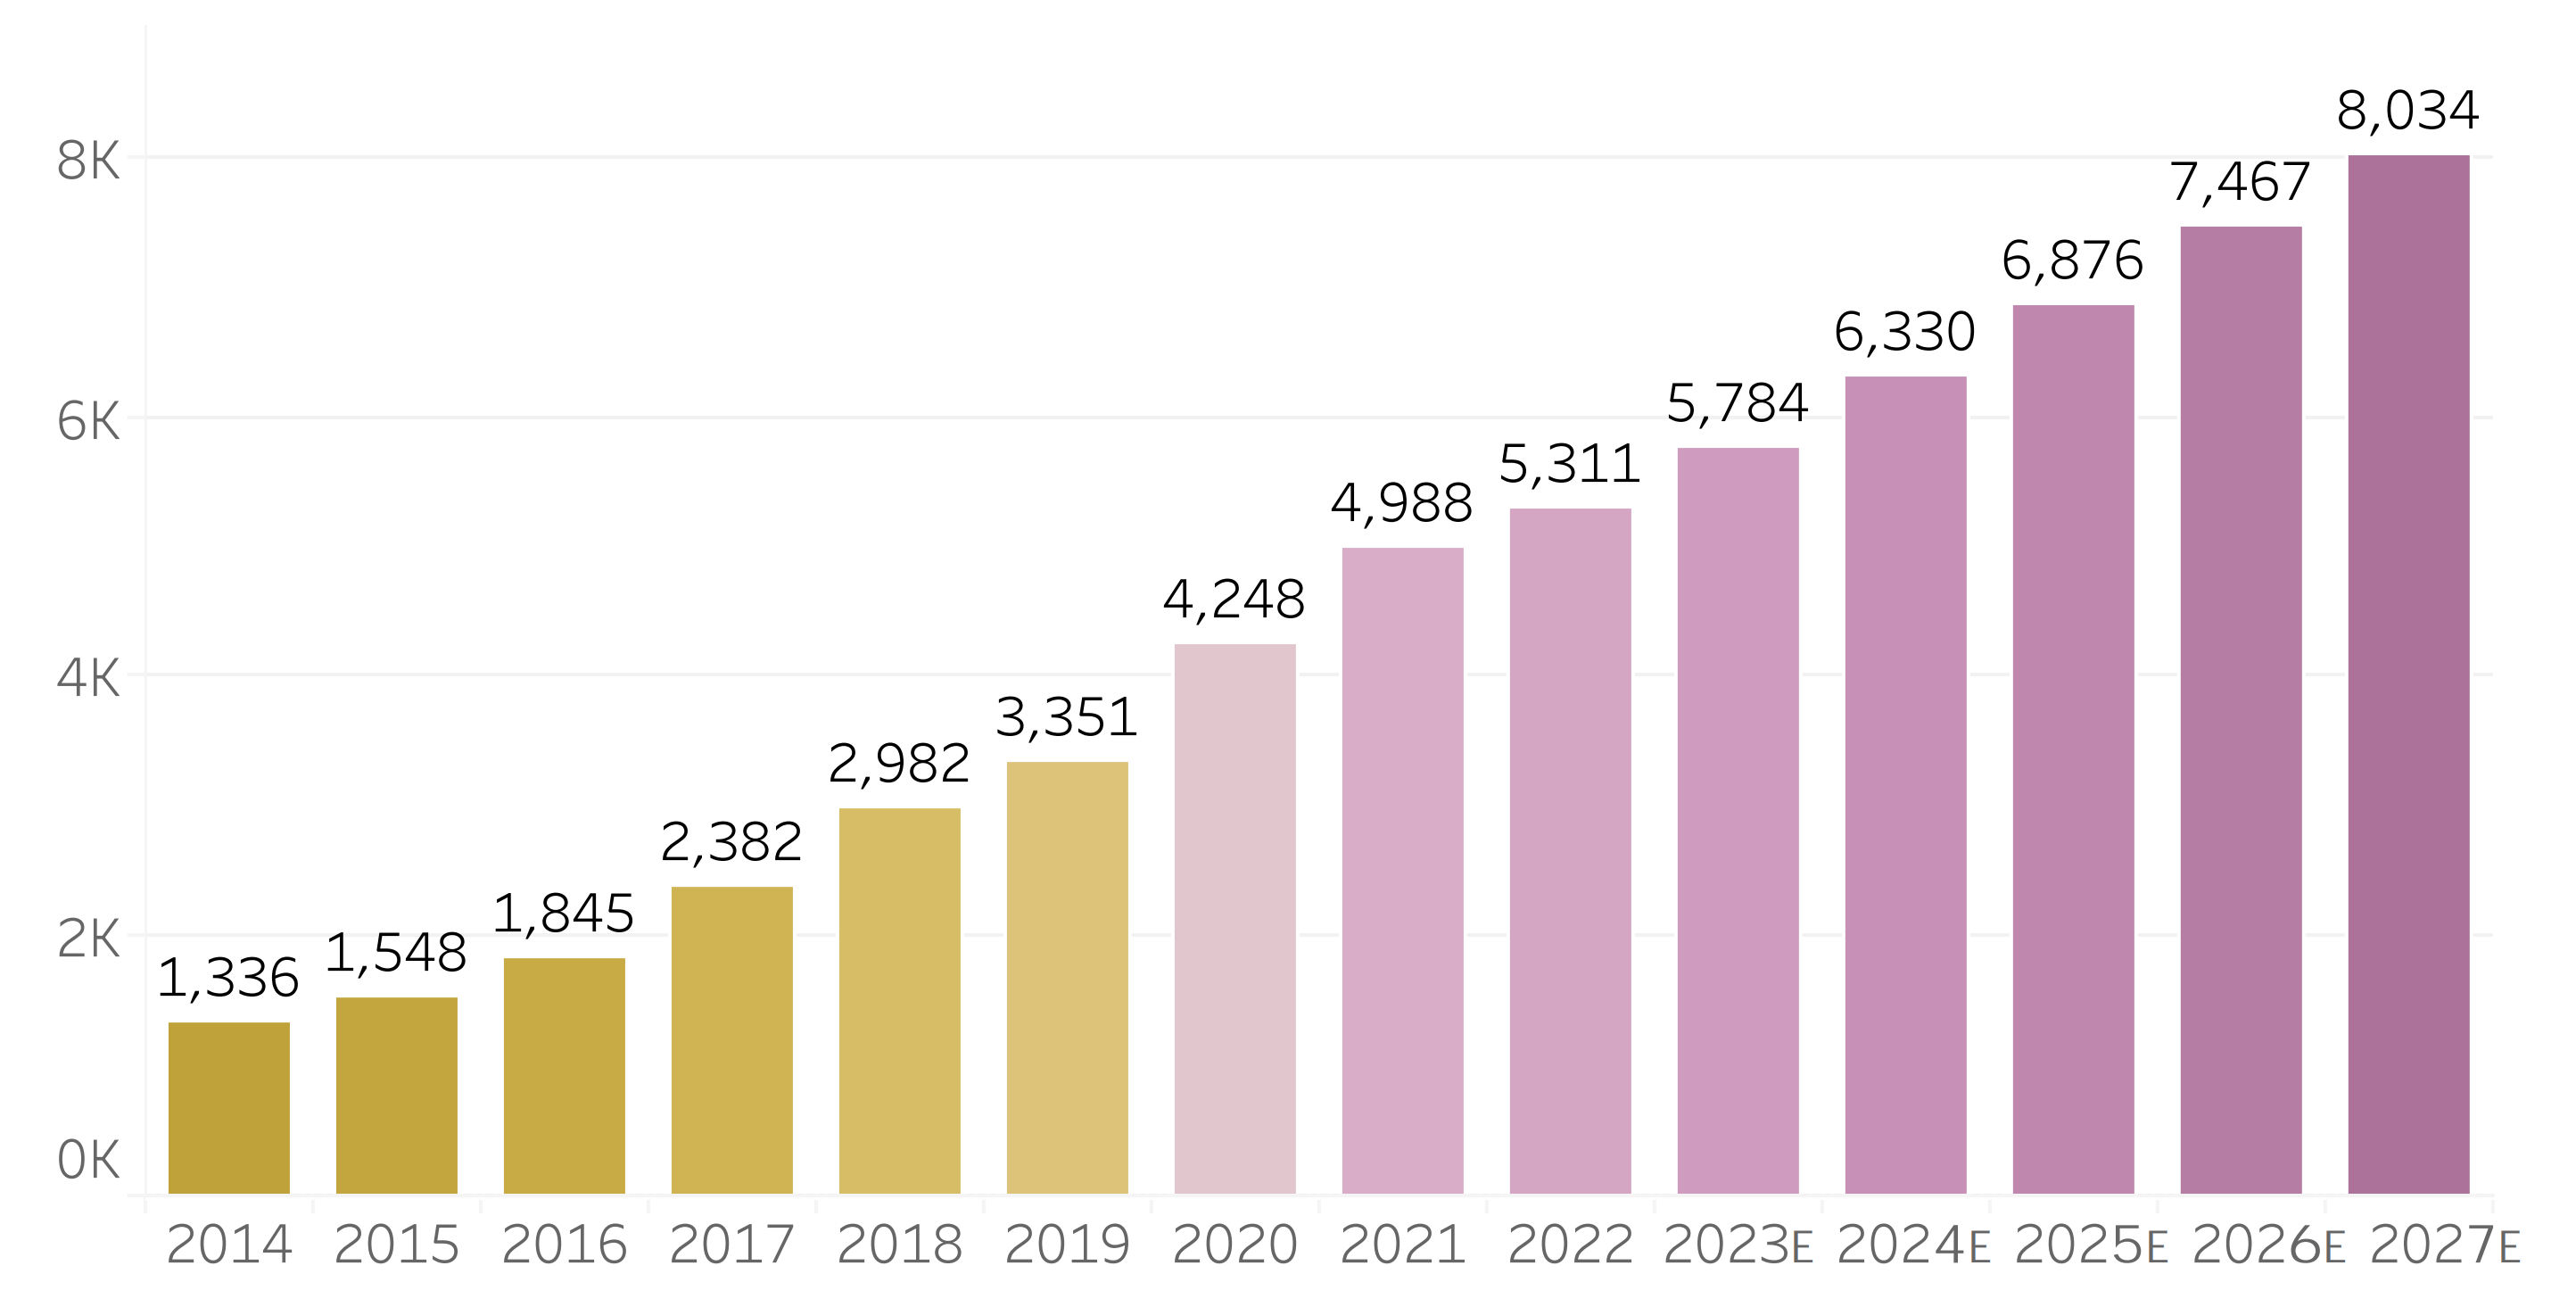
\includegraphics[width=0.8\textwidth]{Images/2.png}
    \caption{2014 - 2027(预测)年全球零售电子商务销售额(单位:十亿美元).(来源:\cite{2})}
    \label{flow}
\end{figure}

如今,这个已经成熟的市场主要涉及企业对企业(B2B)、企业对消费者(B2C)、消费者对消费者(C2C)三种贸易模式。B2B模式一度占据半壁江山,在2022年,全球B2B以市场价值20.4万亿美元超B2C市场价值的五倍多,估计在2027年将达到37.1万亿美元\cite{1}。

\begin{itemize}
    \item \textbf{B2B电商贸易市场} \\
    B2B(Business-to-Business)是企业间的服务或商品互联网交易行为,通常是大额订单交易,自然会集中在经济快速增长且制造业和供应链发达的地区。据AgileIntel Research和Statista报告\cite{1},亚太地区在2022年以超过78\%的份额占据了全球B2B电商市场的主导位置,这一数据也预计在2027年增长到80\%。中东地区近年持续处于高速增长的阶段,预估2023至2027年商品销售总额复合年增长率达24.6\%,远超同时期亚太地区预估的10.0\%。
    \item \textbf{B2C电商贸易市场} \\
    B2C(Business-to-Customer)是企业和私人消费者之间的的服务或商品互联网交易行为,它的最直观解读就是在线零售,交易方的一端从企业变为个人。实际上,现在的B2B正在转向B2E(Business-to-Everyone)模式,也就是说,B2B和B2C的界限变得模糊了,如2020年由ABB India发布的eMart就是一个既支持B2B又支持B2C的在线市场门户网站\cite{1}。单看B2C市场,时尚行业目前为止拥有最大的细分市场\cite{3},但这一趋势似乎并不持久,根据Worldwide的数据和Statista的预测\cite{4},2026年食品行业收入将几乎与时尚行业持平,到2027年时,食品行业将处于领先地位,并在2029年达到1.23万亿美元。
    \item \textbf{C2C电商贸易市场} \\
    C2C(Customer-to-Customer)是两个私人用户之间的的服务或商品互联网交易行为,它相较于B2B和B2C的市场规模则更小,但灵活度更高,也能给用户提供更多元化的购物体验,其中最具代表性的就是二手交易市场。Statista近一年的调查数据\cite{5}显示,欧盟国家中二手购买者占比甚至超过了50\%,在英国,这一数值甚至达到了接近三分之二。据估计,2026年欧盟国家的时装和美容产品线上二手市场规模将达到214亿欧元。自COVID-19以来,由于经济压力,更多人开始寻求价格较低的商品,二手商品就成为一个实惠的选择,而随着群众对环境和可持续发展问题关注度的增加,环保主义消费者也开始选择这一品类。
\end{itemize}



\begin{figure}[htbp!]
    \centering
    \begin{minipage}{0.27\textwidth}
        \centering
        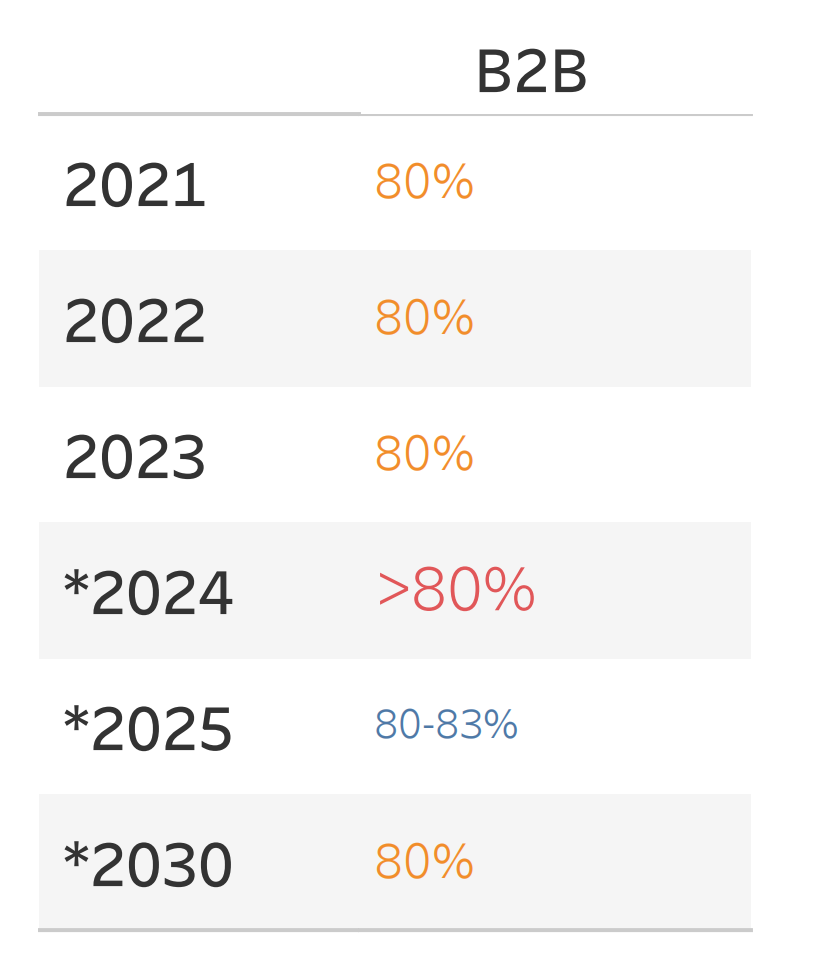
\includegraphics[width=\textwidth]{Images/111_00.png}
    \end{minipage}
    \hfill
    \begin{minipage}{0.27\textwidth}
        \centering
        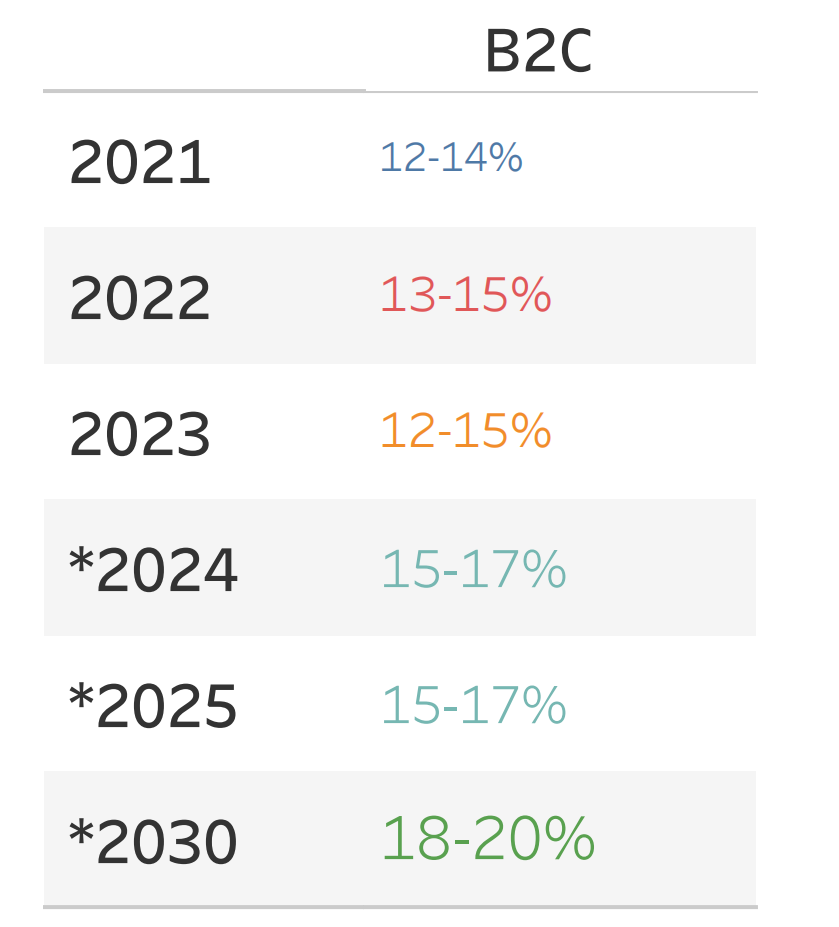
\includegraphics[width=\textwidth]{Images/222_00.png}
    \end{minipage}
    \hfill
    \begin{minipage}{0.26\textwidth}
        \centering
        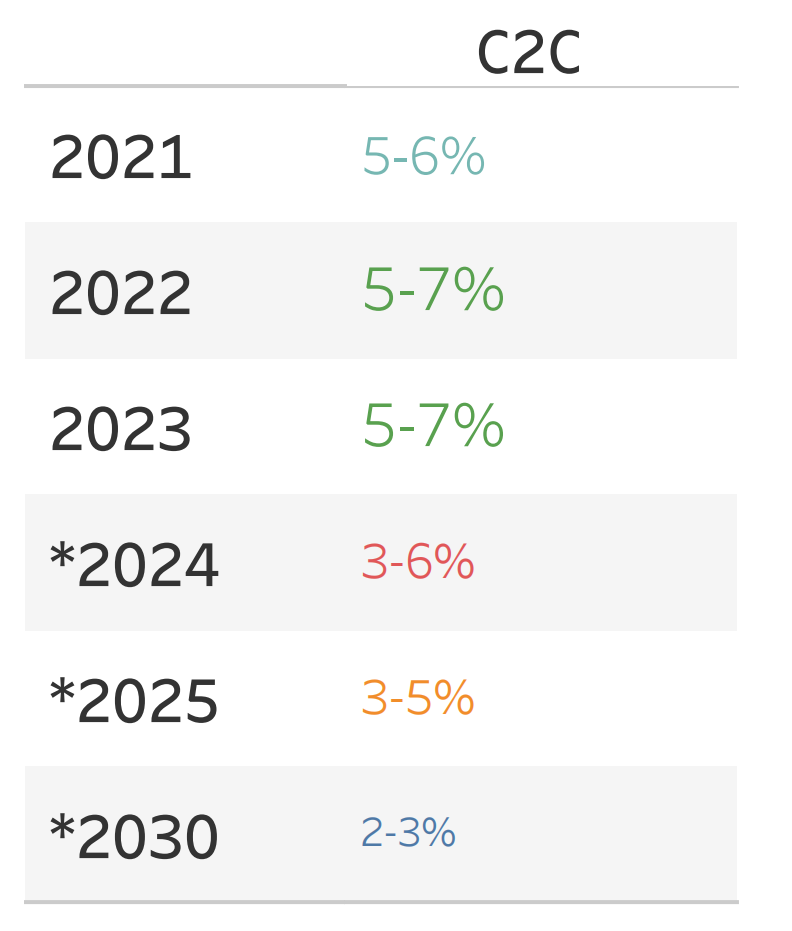
\includegraphics[width=\textwidth]{Images/333_00.png}
    \end{minipage}
    \caption{2021-2025各电商模式年度市场占比.(来源:\cite{21,22})}
    \label{all}
\end{figure}
从全球的角度整体来看,B2B、B2C 和 C2C 市场占比在近年内变化不大,它们的市场份额基本保持相对稳定,未来大致也不会有巨大变动(见图(\ref{all}))。Grand View Reasearch和Nova One Advisor最近发布的报告中都指出,B2B 一直占据全球电商市场的绝大部分,约 80\% 左右,这种主导地位预计会延续到 2030 年。B2C在2030年或将在市场占比上大幅提升至 18-20\%,其市场规模可能达到 31万亿美元,技术进步(如增强现实、虚拟现实等)将推动B2C的进一步扩展。


\subsection{跨境电商地区发展及主要市场}
当卖家与顾客分处不同关境时,这种交易就是跨境贸易,也称跨境电商,是电子商务的一种。实际上,跨境电商在各地区电商市场占比不高,在大部分国家甚至占不到十分之一,见图(\ref{fl})。

\begin{figure}[htbp!]
    \centering
    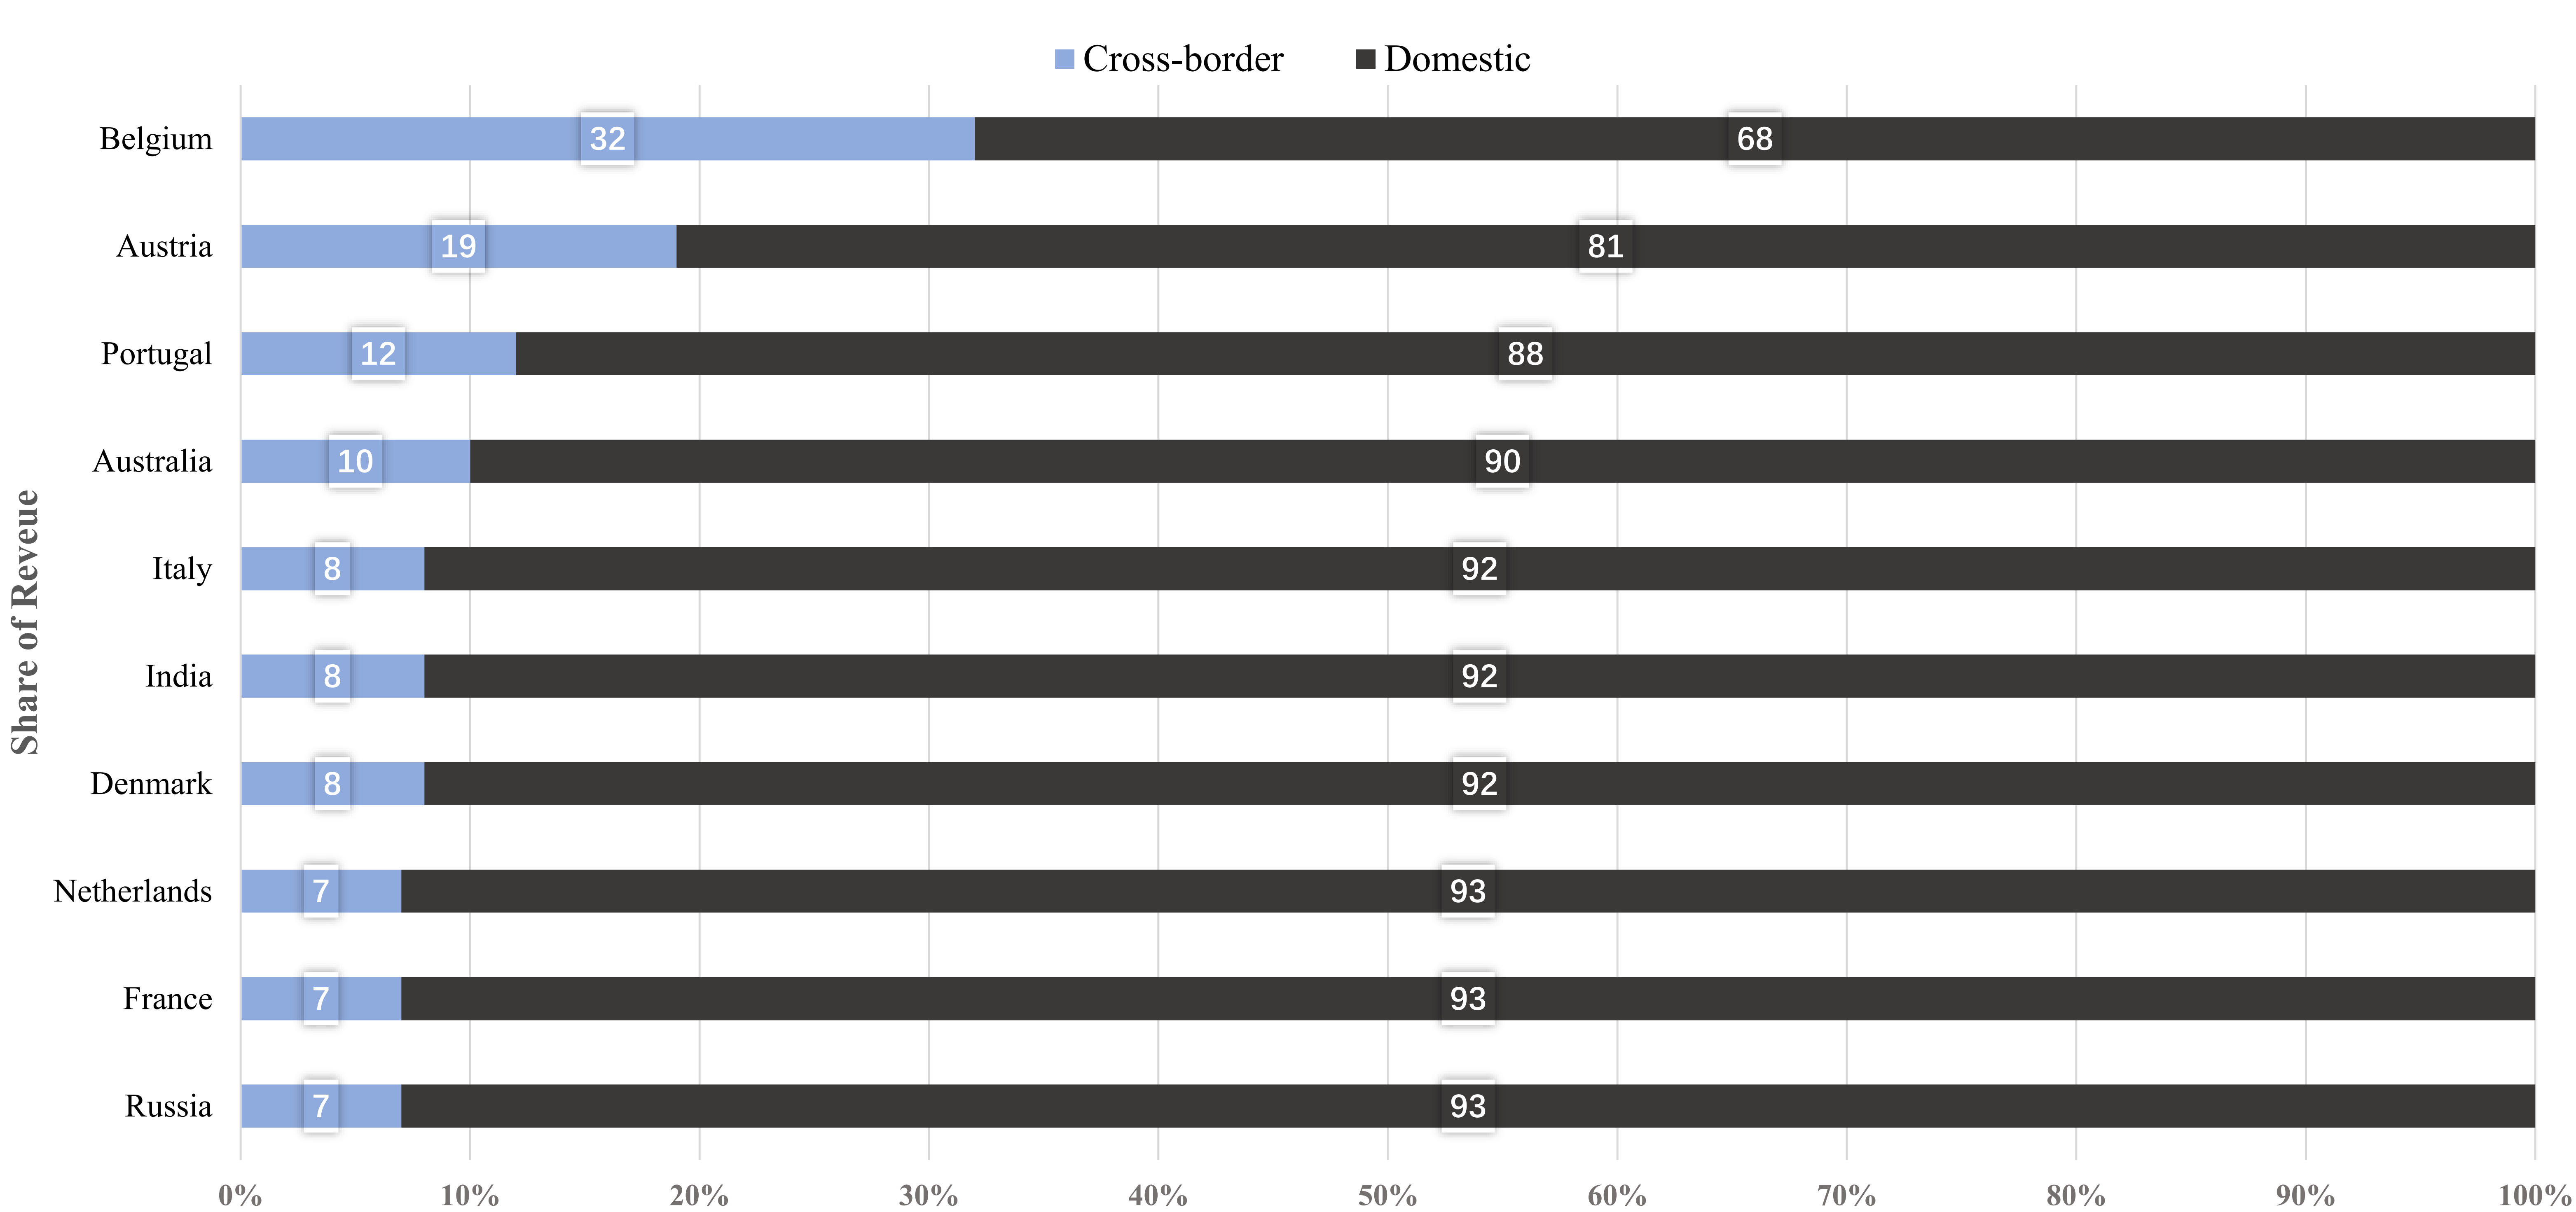
\includegraphics[width=1\textwidth]{Images/1_00.png}
    \caption{2023年各国国内和跨境电子商务活动收入分布(按降序排列).(来源:\cite{6})}
    \label{fl}
\end{figure}

虽然目前占据份额不大,但它正在蓬勃发展,Yahoo Finance的报告\cite{7}指出,2023年跨境电商市场价值为28307亿美元,预计到2032年将达到164549亿美元,在2024年至2032年的预测期内,复合年增长率为21.6\%,World Bank也做出了类似的判断。报告同时指出,服装和配饰是跨境电商中最受欢迎的商品,笔记本电脑等电子产品也很受欢迎,排在第三位的是美容和个人护理产品,家居产品需求也出现激增,跨境交易平台为消费者提供了“异域风情”选择途径。值得注意的是,去年的交易产品类型以实体产品为主,占比高达97\% \cite{6},虚拟产品市场十分紧缩。

Statista \cite{6}、Yahoo Finance \cite{7}和Facts \& Factors \cite{9}给出了几个主要地区的市场发展趋势:
\begin{itemize}
    \item \textbf{亚洲跨境电商市场.} \\
    该地区庞大的消费基础占了优势,且由于印度、中国、日本和韩国等国对国际产品的需求不断增长,预计亚太地区的B2C跨境电商市场在2023至2032年内较其他地区有更高的增长率,其中,印度将成为该地区内增长最快的市场。中国是最大的快时尚连锁零售商之一Shein的所在地,目前是该领域最大的创收品牌之一。虽然中国的跨境电商交易额年增长率自2020年的19.04\%跌落到了2023年的7.32\%,但它仍然是最受欢迎的海外网购市场,也是是全球大多数消费者最后一次跨境网购的市场。2022年,美国消费者在网上购买的2701亿美元跨境零售商品中,有49\%都来自中国,还有12\%来自英国。
    
    \item \textbf{欧洲跨境电商市场.} \\
    欧洲市场在COVID-19后产生了奇怪的波动,德国销售额占比从2019年的2\%上升到了2022年的14\%,而英国则从13\%下降到了10\%。2023年,德国是第二最受欢迎的海外网购市场,它在消费者最近一次跨境网购中占比13\%,仅次于中国。总的来说,预计第三方(通常是中国)卖家所占份额将不断增加的混合市场将推动该地区商品交易总额的增长。

    \item \textbf{北美跨境电商市场.} \\
    2022年,北美B2C跨境电商市场在占主导地位(45.8\%),加拿大的市场则是该地区增长最快的。墨西哥的跨境网上购物份额最高,为6\%。调查数据显示,60\%的墨西哥和加拿大受访者在国际网站购物,而美国受访者中这一比例仅为三分之一。大多数美国在线购物者更喜欢从当地商家或本土电商那里购买产品。

    \item \textbf{中东、非洲和拉丁美洲跨境电商市场.} \\
    这三个地区的制造企业、零售商和物流服务提供商比世界其他地区的企业依赖跨境电商。在非洲和拉丁美洲,33.8\%的电商销售来自跨境交易,而在中东地区,这个百分比数值为29.3\%。近年,年轻人口不断增长,电商部门发展迅速,这三个地区的跨境电商市场预计将显著扩张。
    
\end{itemize}

截止2023年,亚洲毋庸置疑仍然是最大的市场,占总市场份额的88\%,其中中国市场是领头羊,它在2022年的发展指数排名中以71.4分位居榜首\cite{7}。B2C贸易模式在全球跨境电商中贡献突出(占69.8\%),在中国,这一比例在2023年达到了81.3\%,余下的则全部属于C2C \cite{6}。


\subsection{跨境电商驱动因素与竞争局势}
全球化政策的加深和快速前进的技术创新就如一把凸透镜,不断将跨境电商市场放大。自 20 世纪 90 年代以来,随着多边贸易协议的达成,例如世界贸易组织(WTO)的正式成立,跨国贸易壁垒大幅减少;支付宝和 PayPal 能够支持多币种交易,直接简化了跨境交易流程;区块链技术也带来了革命性变变革,如IBM 和 Maersk 合作开发的 TradeLens,它可以追踪和管理全球贸易中的物流信息\cite{8}。此外,大数据和AI技术的发展可以更好揭示消费者的偏好、购买模式,通过分析点击数据生成偏好推荐,提高购买转化率。如迪卡侬(Decathlon)曾经在2018年于芬兰推出线上商店,使用机器学习技术实时分析和监控客户行为以推荐产品,最终他们的收入增长了10.7\%;国际珠宝公司潘多拉(Pandora)则提供了虚拟试戴技术,也将他们的收益显著提高\cite{3}。最优化个性化购物体验已经成为许多涉足跨境电商活动的大企业的未来发展趋势\cite{7}。

有市场的地方就有竞争,跨境电商中的“领头玩家”有Alibaba、AirBridgeCargo Airlines、AliExpress、Amazon、ASOS、BigCommerce、eBay、Eunimart Multichannel、Jagged Peak、JD、Pitney Bowes、Tmall、Vipshop、Zalando(按首字母排序)等\cite{9}。邓白氏(Dun \& Bradstreet)2023年全球跨境电商综合评估前五分别为Walmart、Amazon、Home Depot、Alibaba、JD \cite{10}。

不妨把目光放到Walmart、Amazon、Alibaba最具有代表性的三巨头身上。Walmart以实体店起家,以低廉的商品价格和广泛的商品选择在全球拥有数千家商店,其电商平台推出后整合了在线和实体零售业务,为顾客提供了无缝的购物体验,在2022年也推出了“Walmart+”订阅服务以对抗亚马逊的“Amazon Prime”服务\cite{11};Amazon则是抢占电商市场的先锋,它作为第三方从创立起就在线上平台连接买家和卖家(B2C模式),且十分重视技术创新与智能化来提升用户体验,是网上购物的首选\cite{12};Alibaba在推出时就注重的是B2B模式,是全球领先的批发市场,连接着全球数百万买家和供应商,其集团下的天猫平台是B2C模式,而另一平台淘宝则是C2C模式,它同时关注新兴技术,是人工智能和智能物流发展的先驱。Alibaba在今年7月发布的报告\cite{11}中称Amazon的两个最大竞争对手就是Alibaba和Walmart。具体而言,Walmart的“Click \& Collect”服务是整合线上线下优势的直观体现,其支持消费者线上购买、线下门店取货,极大节省配送时间和费用;Amazon的“Fulfillment by Amazon (FBA)”服务则允许第三方卖家将库存存储在亚马逊的仓库中,使用亚马逊物流网络配送,以此直接提升卖家的配送效率和顾客体验;Alibaba则推行“天猫双11”全球购物盛会,并通过蚂蚁金服(Ant Group)推动了全球支付创新,同时也投资Lazada以扩大其东南亚地区市场来与Amazon和Walmart竞争。

\subsubsection{综合各平台报告的Walmart、Amazon、Alibaba竞争优劣势简析}
\begin{itemize}
    \item \textbf{Walmart vs Amazon.} \\
    沃尔玛凭借其广泛的实体店网络和低价战略,能够在全球范围内通过规模效应实现低成本运营,这使其在价格敏感的市场中具有竞争优势。他们也有强大的供应链管理和物流系统确保高效的库存管理和产品配送(来源:Harvard Business Review)。但电商业务起步更晚,尽管近年来有所增长,但其线上平台的用户基础较弱,运营经验也不足(来源:Forbes)。

    相比之下,亚马逊在技术创新方面具有显著优势,包括云计算、人工智能和物流自动化等领域的领先地位(来源:Amazon Annual Report)。亚马逊的产品多样性和全球供应链支持其强大的跨境电商业务,使其能够在国际市场上提供个性化的购物体验(来源:The Wall Street Journal),他们也在用户满意度的提升上下足了功夫。然而,亚马逊面临着更高的价格压力和市场监管,这是其市场竞争战略和扩张速度的难关(来源:Financial Times)。
    
    \item \textbf{Amazon vs Alibaba.} \\
    亚马逊凭借其全球市场覆盖能力和技术驱动的运营优势,能够在多个国家和地区建立强大的市场份额,创新个性化推荐和快速配送也能成功留下许多使用者(来源:Amazon Annual Report、TechCrunch)。相对于阿里巴巴集团,它在全球跨境贸易市场的主导地位仍然是不可撼动的,但如果聚焦到中国这个潜力无限的市场呢?亚马逊的光芒则暗淡不少了。

    但就中国市场而言,阿里巴巴通过其多元化的电商平台和本土优势占据了亚洲电商市场的重要地位,淘宝、天猫、阿里云等形成了一个强大的生态系统(来源:China Daily),得益于达摩院(DAMO Academy)的成立,其技术发展也不逊于亚马逊。但在国际扩展中,阿里巴巴却还是面临着不同文化和市场需求的适应问题(来源:The Economist)。
    
    \item \textbf{Alibaba vs Walmart.} \\
    阿里巴巴凭借其强大的电商平台和在线支付系统,如支付宝,促进了交易的便捷性,并利用中国市场的经济规模(也就是近十年的高速进步)实现了业务的快速增长(来源:Alibaba Group),但与全球各个地区本地平台竞争却因进入较晚吃了亏(来源:The Financial Times)。其旗下的盒马鲜生(Hema)作为一个集超市、餐饮和配送于一体的混合零售商店在中国各大城市取得了显著成功,但尚未、也很难在其他国家开设门店。

    沃尔玛依托其广泛且雄厚的实体店网络,拥有全球超过10,000家门店,包括超级市场、折扣店和仓储俱乐部,他们也为线上订单提供了多样化的配送和取货选项(来源:Walmart Annual Report)。其低价策略在全球范围内有效,能够吸引价格敏感的消费者(来源:Harvard Business Review),虽然亚洲生产成本低廉,但在这一策略下阿里巴巴并不占优势。
    
\end{itemize}

\begin{figure}[htbp!]
    \centering
    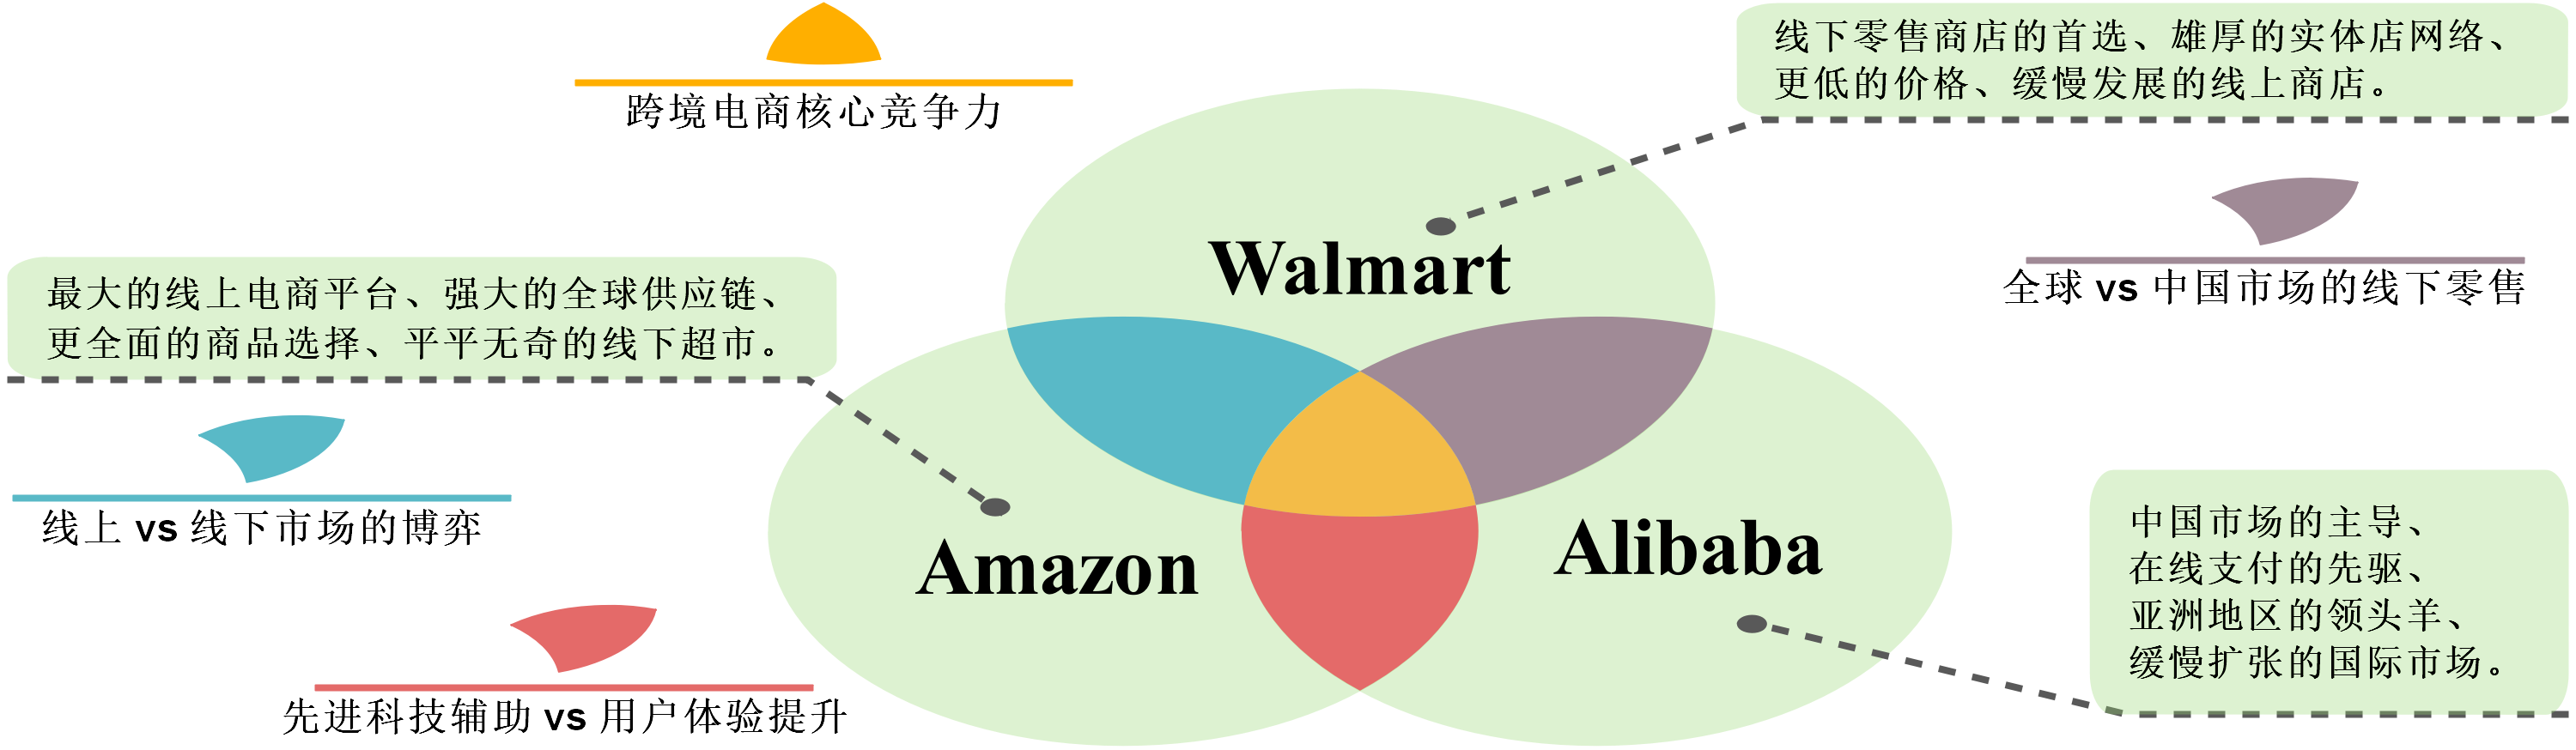
\includegraphics[width=0.93\textwidth]{Images/10.png}
    \label{flow}
\end{figure}

\subsubsection{技术创新为竞争局势带来的动态影响}
“AI战”在各个市场上都不是一个陌生的词汇。在上面提到的三家企业中,亚马逊的表现尤为突出。在今年3月的一篇报道\cite{24}中,亚马逊企业风险投资部门负责人Franziska Bossart透露,亚马逊今年正在以10亿美元的工业创新基金加大对融合人工智能和机器人技术公司的投资,以提升整个物流网络的效率。他们已经进行了十二项投资,其中一项用于Mantis Robotics与人类工作的机械臂的开发。最近,亚马逊将首席工程师的小狗Rufus “带回了办公室”,作为其人工智能数字购物助理的名称;同时,沃尔玛并不示弱,推出了自己的人工智能数字购物助理My Assistant,Forbes称人工智能是这场“2.0”零售革命的核心\cite{25}。阿里巴巴则没有过多参与二者之间的竞争,一直将目光放在潜力满满的亚洲市场。

送货服务也已经迎来智能技术更新迭代阶段。亚马逊的 Prime 免费送货服务一直是其与沃尔玛竞争中关键的差异化因素,目前,沃尔玛正在建设五个新的高科技易腐品配送中心,并扩建四个传统易腐品中心,每个站点增加 50 万平方英尺的自动化设施,以提高新鲜产品的产能。过去一年,沃尔玛在美国公司共计有 44 亿件商品在当天或次日送达,其中约 20\% 在三小时内送达,沃尔玛逐渐增强的配送实力无疑会对亚马逊造成一些冲击\cite{26}。得益于中国本身高度发达的物流网络,阿里巴巴并不需要在这方面下许多功夫。

今年,沃尔玛将重心放在了用户体验。iOS 用户现在可以使用全新的生成式 AI(GenAI),更加智能地进行搜索,例如,用户可以直接搜索“足球观赛派对”,系统会根据具体场景推荐薯条、鸡翅、饮料和大屏电视等,而不需要分开搜索各个物品。新的 InHome 补货功能能够智能地在合适的时间为用户的网上购物车补充商品,并将商品直接送到用户的厨房或车库冰箱。与此同时,新推出的Shop with Friends 社交购物平台可以让用户与朋友分享AR试穿的服装,并实时获得反馈\cite{27}。今年6月初他们宣布,到2026年,2300家门店将全部取消纸质价格标签,化简价格更新流程,花更多的时间服务顾客\cite{28}。沃尔玛正在提升用户体验来与亚马逊的“Prime”服务抗衡。

同年,亚马逊的关注点在科技。7月26日,德勤宣布与亚马逊云科技签署了一项长期战略合作协议,旨在利用亚马逊云科技(如Amazon SageMaker、Amazon Bedrock、Amazon Q和Amazon Braket)帮助全球客户增强其在生成式AI、数据分析和量子计算领域的能力,双方还计划共同建立创新实验室,探索人工通用智能、量子机器学习和自主机器人等前沿技术\cite{29}。四天后,亚马逊在“云科技汽车暨制造与消费电子行业峰会”上宣布正式启动“智能家居与智能产品创新加速计划”\cite{30},他们一直以开创者的身份前进,这个加速计划更或将他们在这个领域的优势持续且高速放大。阿里巴巴曾开发过天猫精灵,但它在市场上似乎并不是十分受欢迎。就在八月,阿里巴巴的电子商务部门淘宝和天猫集团成立了新的“数字技术”公司,他们的目标是和中国企业京东、拼多多和字节跳动旗下的抖音等年轻的在线零售平台竞争,这场战役并没有波及到他们。


\section{亚马逊发展历程}

\subsection{亚马逊的创立与早期发展}
亚马逊在2023年以惊人的1.045万亿美元的市值排名世界第五\cite{13},它一直是市场中强有力的存在,但谁曾想,这样一所大公司是在出租屋的车库中诞生的。1994年7月,杰夫·贝佐斯(Jeff Bezos),一个年轻的普林斯顿大学毕业生以“Cadabra”(abracadabra)的名字创立了它,几个月后,正式改名“Amazon”,不久后,网站正式发布,亚马逊成为了一个在线图书销售平台。

\begin{figure}[htbp!]
    \centering
    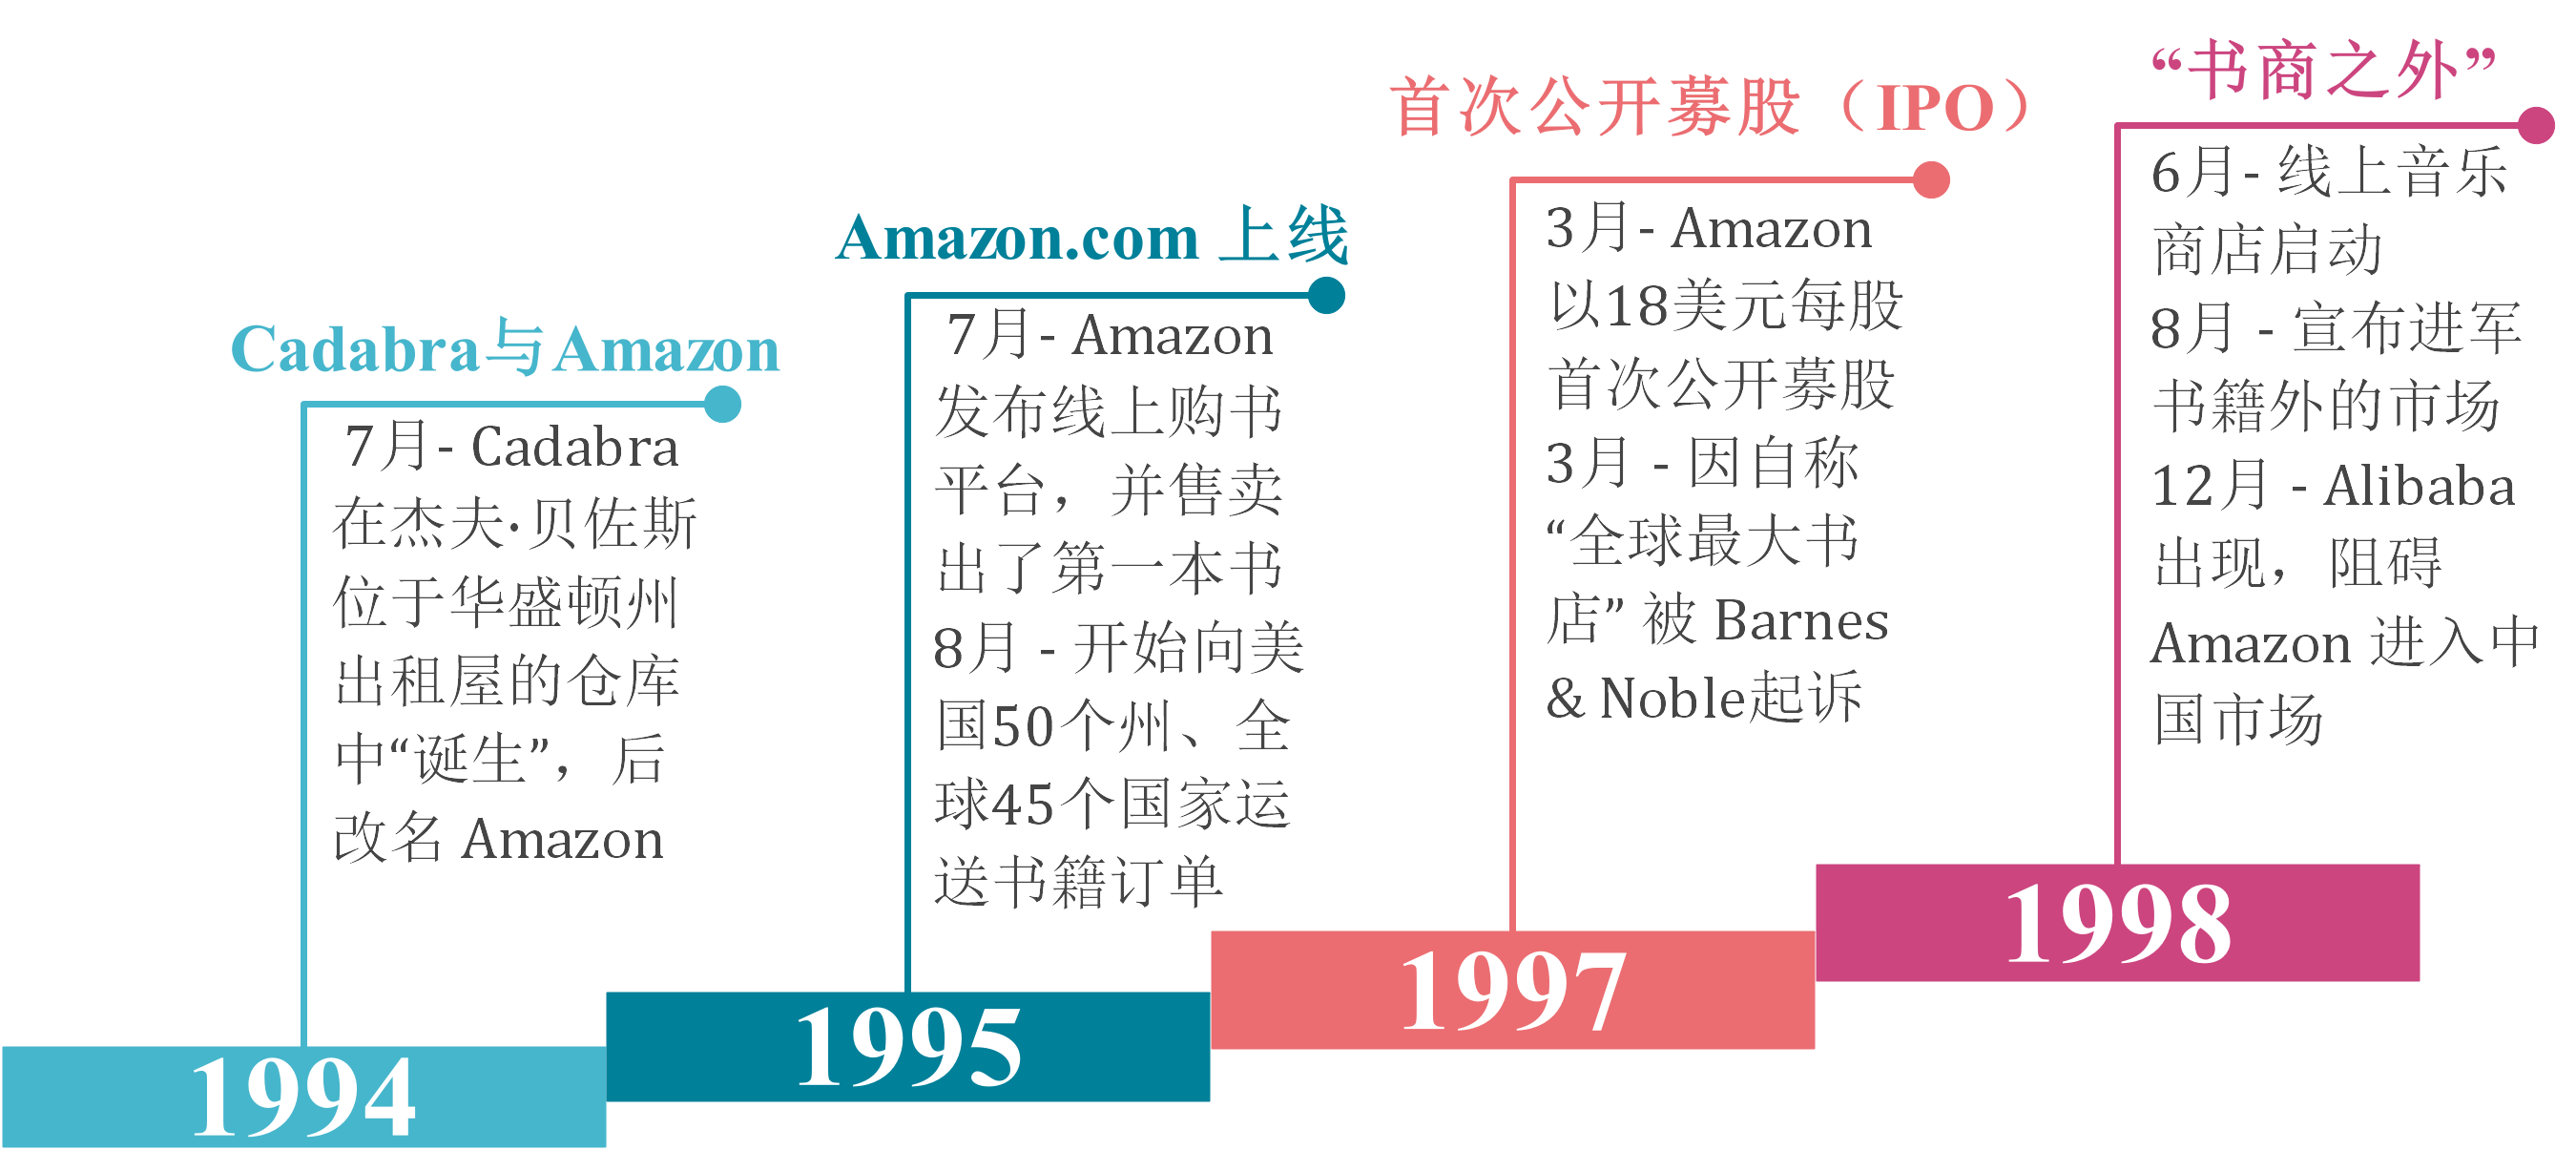
\includegraphics[width=0.9\textwidth]{Images/3.png}
    \caption{早期亚马逊发展时间线(来源:\cite{14,15})}
\end{figure}

2000年前,亚马逊的重点仍在图书,Barns \& Noble还就“全球最大书店”起诉了他们\cite{14}。

\subsection{21世纪的亚马逊}
21世纪初,亚马逊推出了Marketplace,一个允许第三方卖家销售产品的平台,并将自己的公司标志改成了连接字母A和Z的笑脸,代表任何产品都可以在他们这里找到。

\begin{figure}[htbp!]
    \centering
    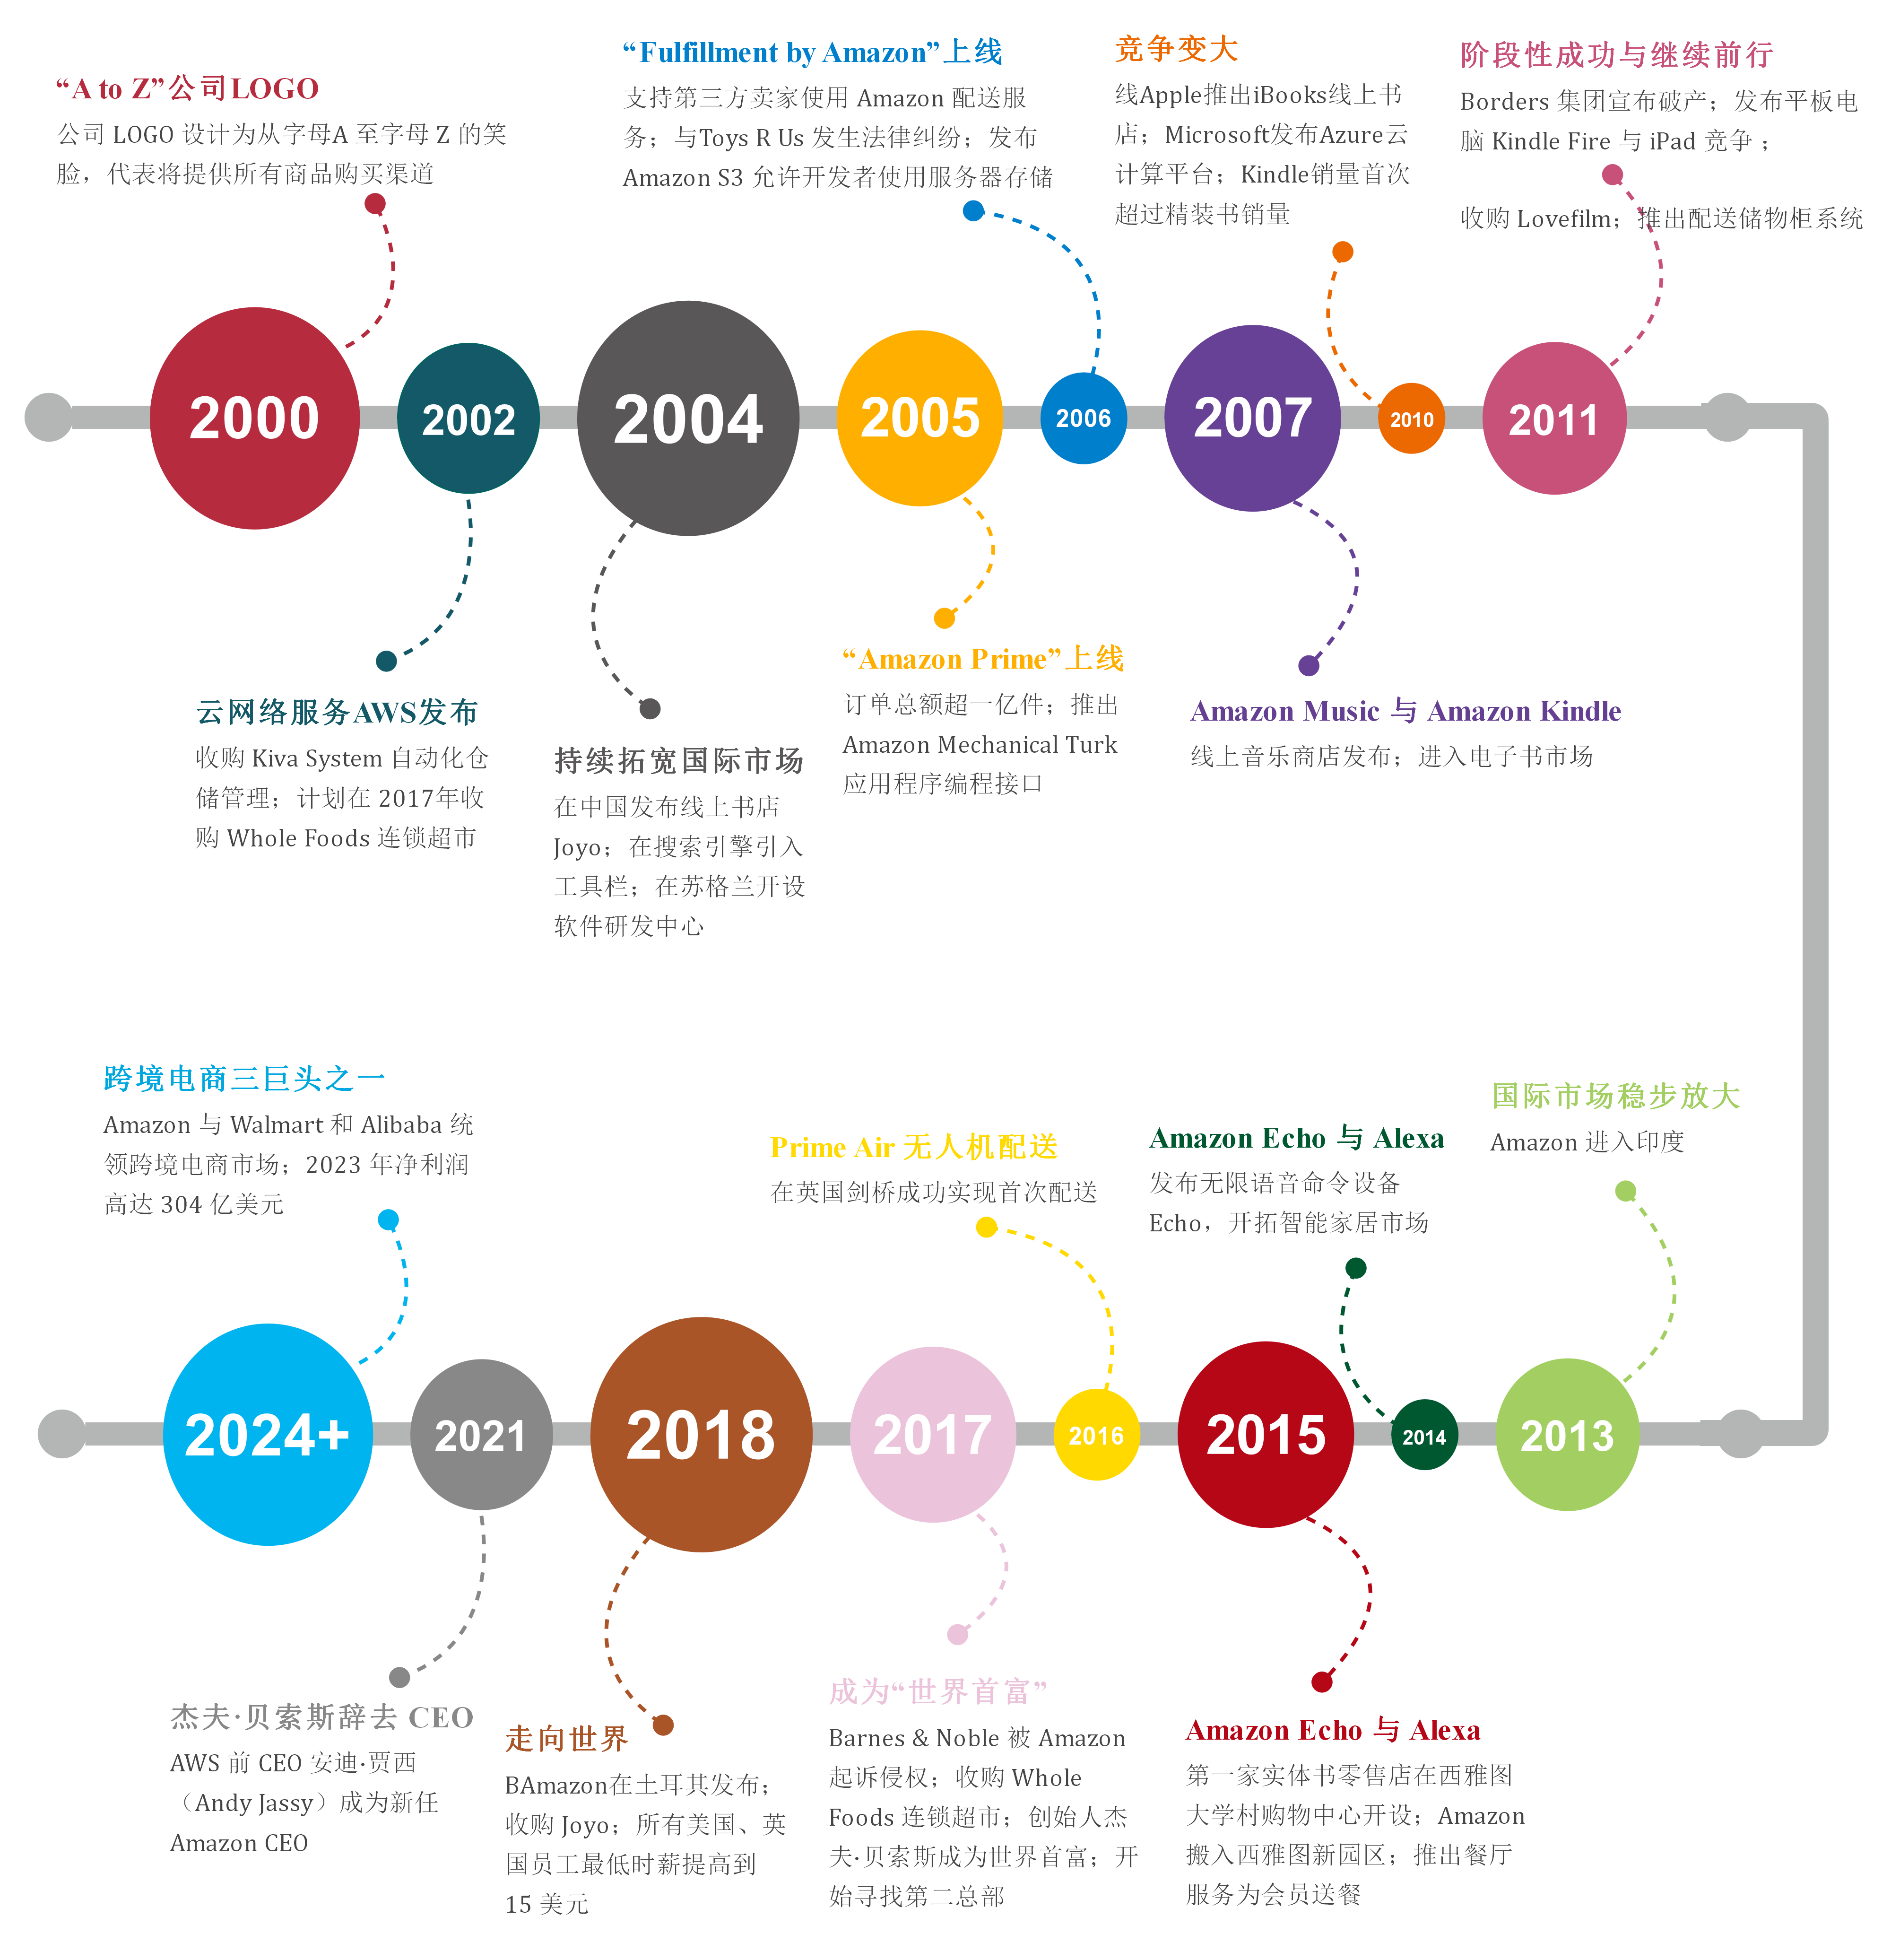
\includegraphics[width=1\textwidth]{Images/4.png}
    \caption{21世纪后亚马逊发展时间线(来源:\cite{14,15})}
\end{figure}

\subsection{关键节点:亚马逊发展历程中的重大事件}
\begin{itemize}
    \item \textbf{1997年的首次公开募股.} \\
    初期,亚马逊一直面临着巨大的现金流压力且持续处于亏损状态,“增长优先于盈利”战略让投资者们一度十分质疑公司的前景。NASDAQ(National Association of Securities Dealers Automated Quotations)给了他们一个机会,1997年,亚马逊以每股18美元的价格首次公开募股(IPO)上市,并筹集到5400万美元。利用这笔钱,从书籍扩展到音乐、电子产品等,亚马逊得以巩固了其作为综合在线零售商的地位,成功渡过了早期生存危机。
    
    \item \textbf{2001年的互联网泡沫与扭亏为盈.} \\
    2000年互联网泡沫破裂,众多互联网公司倒闭,亚马逊也亏损严重。贝索斯立即严格管控成本并提升运营效率(如物流中心优化等)。他关闭了冗余仓库、引入条形码扫描和自动分拣系统缩短订单处理时间、引入了自助式的客户服务提升用户满意度,股价开始稳步回升。    
    
    \item \textbf{2005年的“Amazon Prime”服务推出.} \\
    2000年代中期,市场竞争愈发激烈,面对eBay等其他强劲的电商平台,亚马逊急需提升用户粘性并提高订单频率。“Amazon Prime”服务迅速推动了亚马逊订单量的增长,并且增强了用户的忠诚度。这一服务也成为亚马逊生态系统的核心,为他们长期带来收入的增长。
    
    \item \textbf{2006年的云计算(AWS)推出.} \\ 
    尽管在零售领域成功扩展,但高昂的物流和运营成本使得其盈利微薄,于是贝佐斯转念技术。“Amazon Prime”服务推出仅一年后,AWS(Amazon Web Services)出现了,并为其他企业提供云计算服务。起初这一服务是为了解决亚马逊内部的IT需求,但迅速发展并成为了最赚钱的独立业务之一,推动公司从电商平台转型为全球领先的云计算服务提供商。
    
    \item \textbf{2014年的智能音箱Echo与智能助手Alexa.} \\
    在此之前,与苹果的iPhone和谷歌的Android相比,亚马逊并没有出彩的智能设备,智能家居市场的兴起为他们的进军提供了契机。2014年,亚马逊推出的智能音箱Echo和搭载语音助手Alexa迅速赢得市场青睐,引领了语音助手和智能家居的潮流,也推动了硬件销售。
    
    \item \textbf{2017年的连锁超市Whole Foods收购.} \\
    亚马逊致力电商,难以与传统零售商(如与Walmart)竞争,急需通过线下渠道扩展其市场份额,于是在2017年以137亿美元收购高端连锁超市Whole Foods。这是亚马逊迄今为止最大的一次收购,标志着其正式进入线下零售和生鲜食品市场。依靠Whole Foods提供的庞大线下网络,亚马逊将其物流和配送网络进一步整合,实现了线上和线下业务的协同运作。
    
    \item \textbf{2020年的供应链强化.} \\
    2019年COVID-19爆发,全球封锁和社交隔离措施导致线下消费大幅减少,消费者转向在线购物,贝索斯知道机会来了。面对激增的需求,亚马逊迅速调整运营,增加仓储和配送能力,并强化了其食品杂货和健康产品的供应链,以此巩固了其在全球电商市场的主导地位。
    
\end{itemize}

\subsection{各阶段核心业务与其对亚马逊整体战略的影响}

综合前三节,不难将亚马逊的发展历程分为五个阶段,如图(\ref{sum})所示。

\begin{figure}[htbp!]
    \centering
    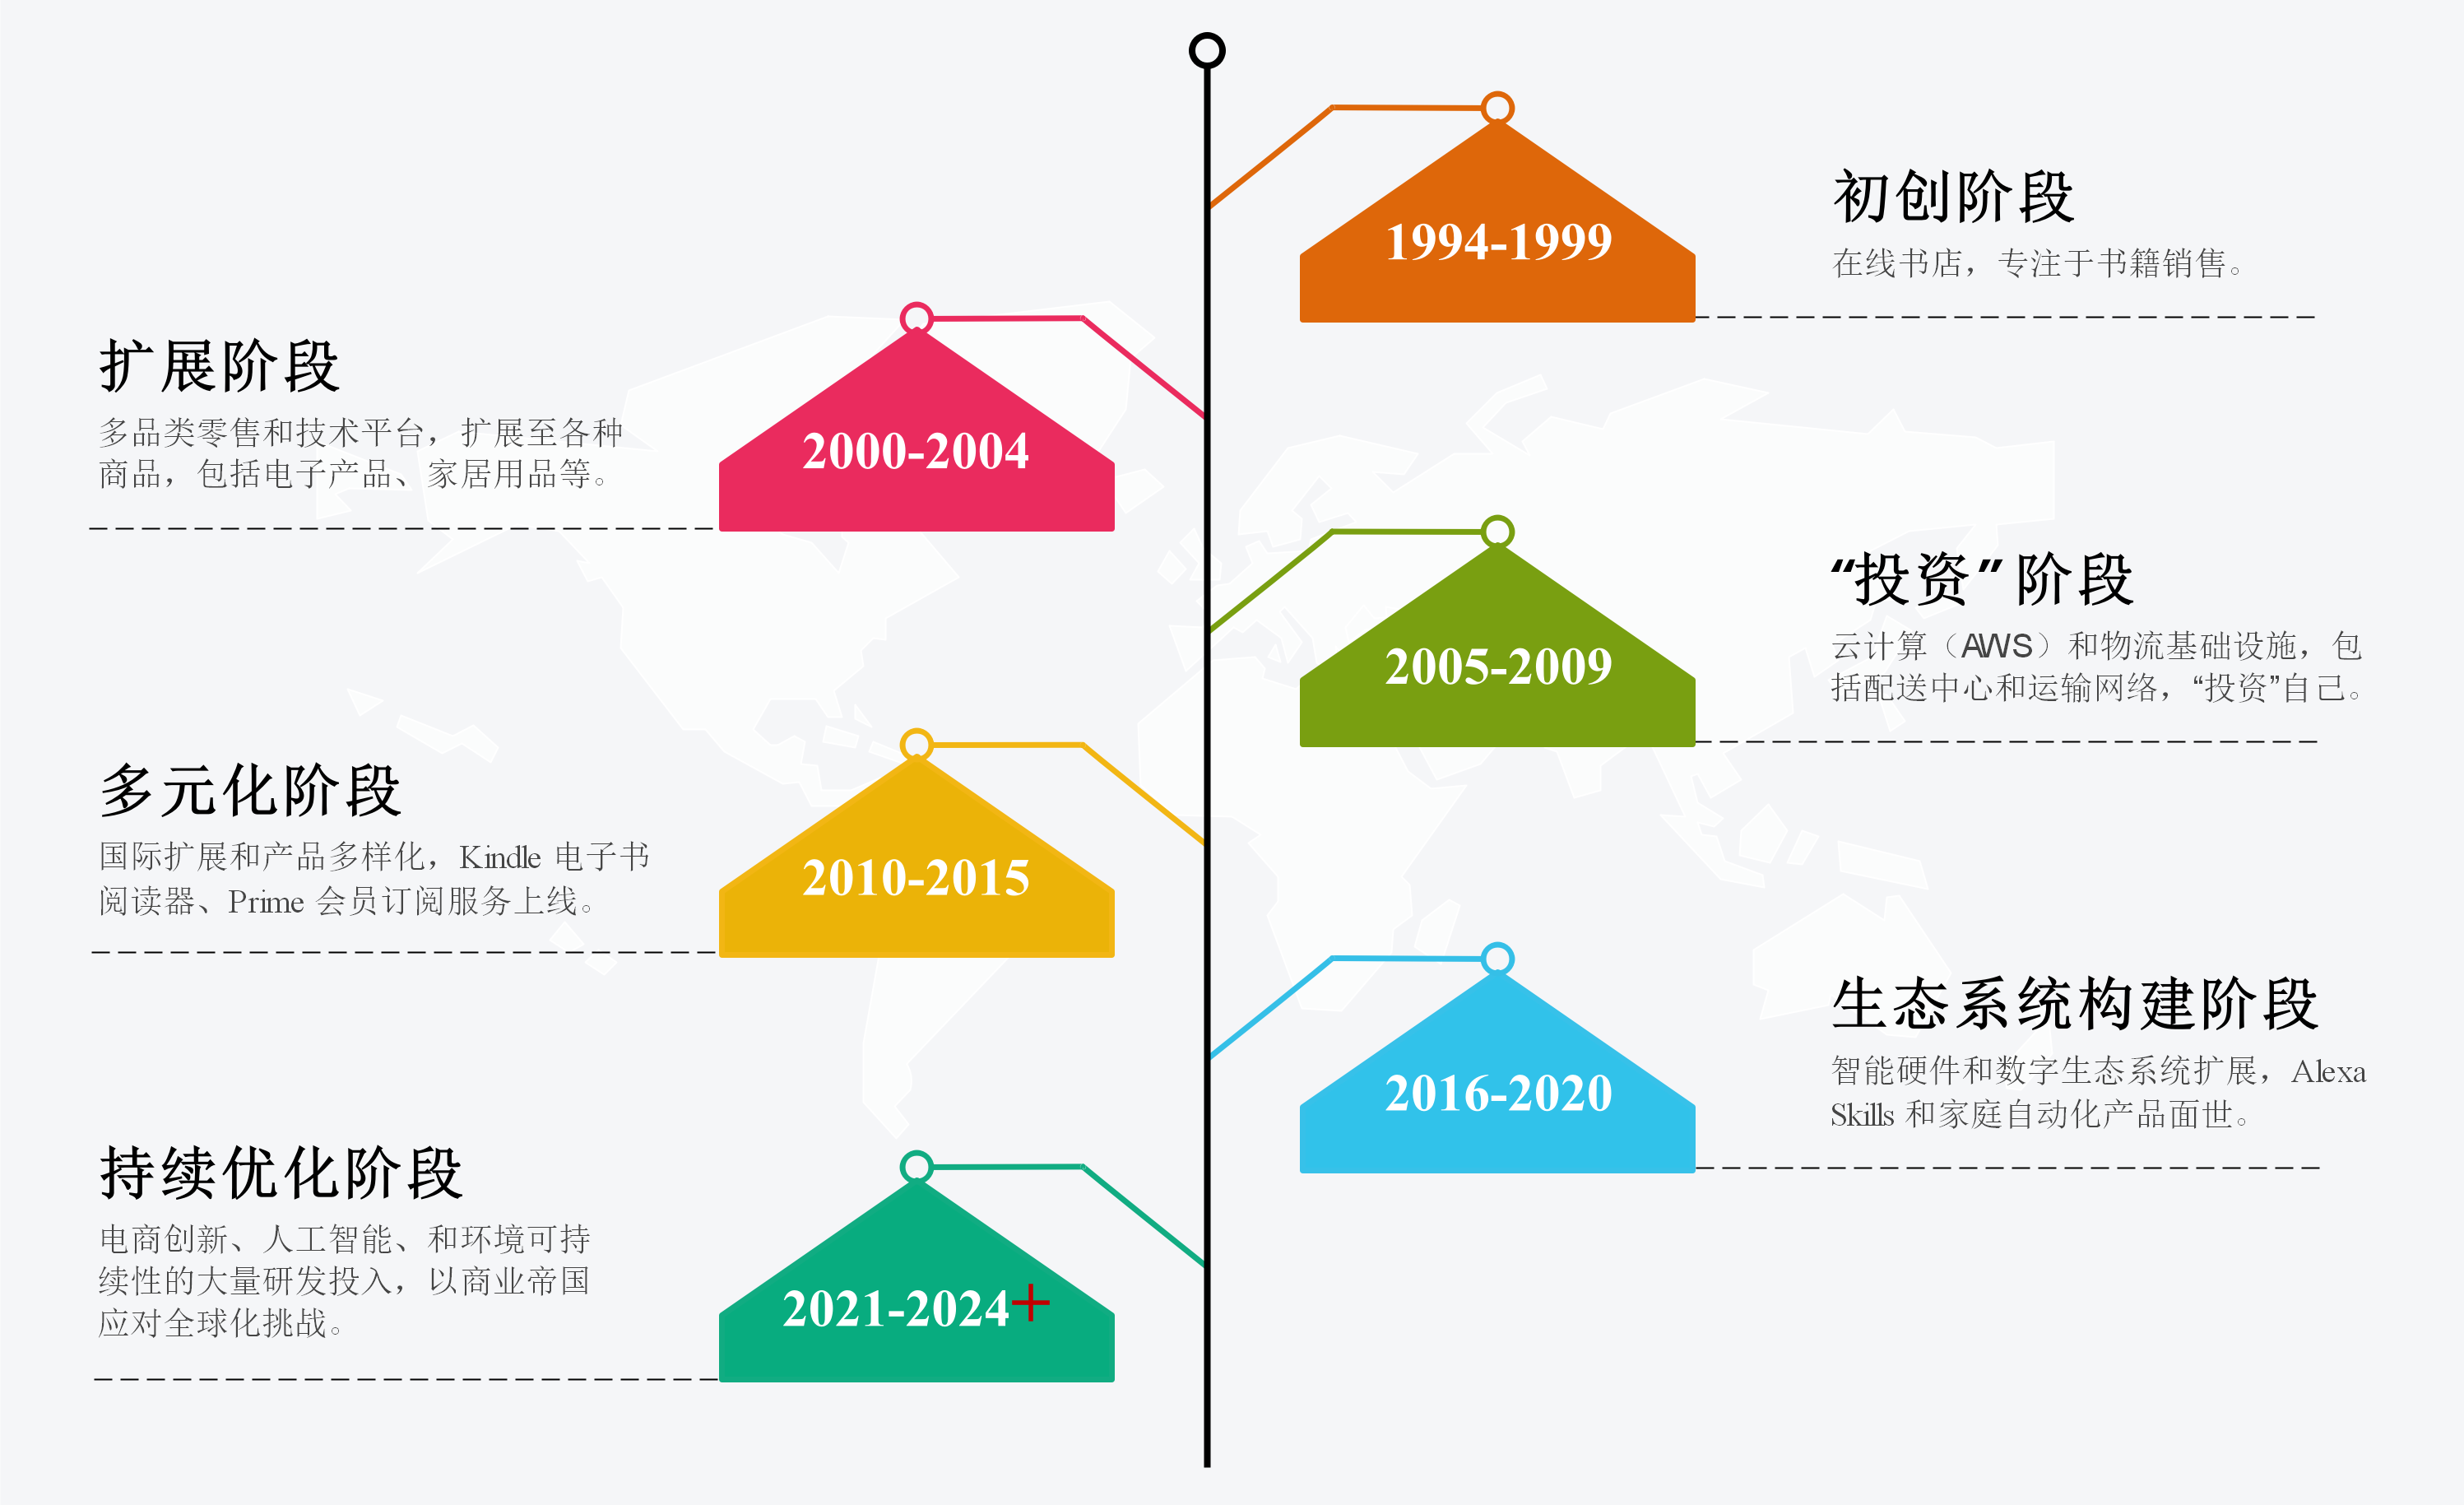
\includegraphics[width=1\textwidth]{Images/Timeline 17.png}
    \caption{亚马逊发展历程小结}
    \label{sum}
\end{figure}

1994至1999年为初创阶段,在这一时期,亚马逊的核心业务是在线书籍销售,这一阶段奠定了亚马逊的电商基础,可以说是未来的“在线零售模式”的一次试水。它以一个初创的身份开始赢得消费者的信任。2000至2004年为扩展阶段,亚马逊的目光不再停留于书籍,而是拓展到音乐、电子产品等,这一阶段的核心业务是推出的Amazon Marketplace,第三方销售平台正式搭建,这个平台的引入进一步丰富了商品种类且拓宽了亚马逊的收入来源与国际声誉,这时其战略目光已经放至全球市场。2005至2009年为“投资”阶段,这里的“投资”指的是亚马逊对自身的投资,在2000年代早期,企业需要自行管理和购买昂贵的服务器、存储设备和网络设施,导致基础设施管理成本极其灵活且差,云计算则可以很好满足开发人员的需求,至此“电商公司”转变为“技术公司” ,这一阶段是亚马逊整体战略变动的关键点。以技术创新商业化,亚马逊也得以扩展其业务版图,且技术的关卡之上,被其他同类型企业超越的风险也就减小了许多。2010至2015年为多元化阶段,亚马逊的战略目标再次回到拓展之上,这一次的拓展则更多放在了特有产品与服务上,在这一阶段推出的Kindle电子书引领了电子书风潮,从未来的视角看来,更加值得称赞的则是其推出的“Prime”会员制,这也是说明更多的中心放在了用户黏着性的巩固之上。2016至2020年为生态系统构建阶段,经过了前几个阶段的发展,亚马逊在这阶段的首要目标就是“融而合之、固而牢之”,在其技术的支撑下,家庭自动化产品进入人们的视野,真正将用户满意度、技术投资、软硬件合并为一。2021年至2024+为持续优化阶段,自从LLM受到重用,亚马逊的战略便转移至技术研发,大量投入资金、投资初创公司等,这似乎是在效仿之前提到的“投资”阶段,但他们的技术又是以各种各样的产品如智能购物车等形式推出,也就是说这一阶段的战略目标不再仅仅是技术,而也是用户黏着度。未来几年亚马逊可能仍会持续以此为目标。




\section{亚马逊主要业务简析}

\subsection{五大主要业务}
根据Statista报告中的数据显示\cite{16},亚马逊有五大主要业务,分别为云计算(AWS)、会员制与订阅服务、在线商店、实体商店、第三方卖家平台。

\begin{figure}[htbp!]
    \begin{minipage}[t]{0.55\textwidth}
        \centering
        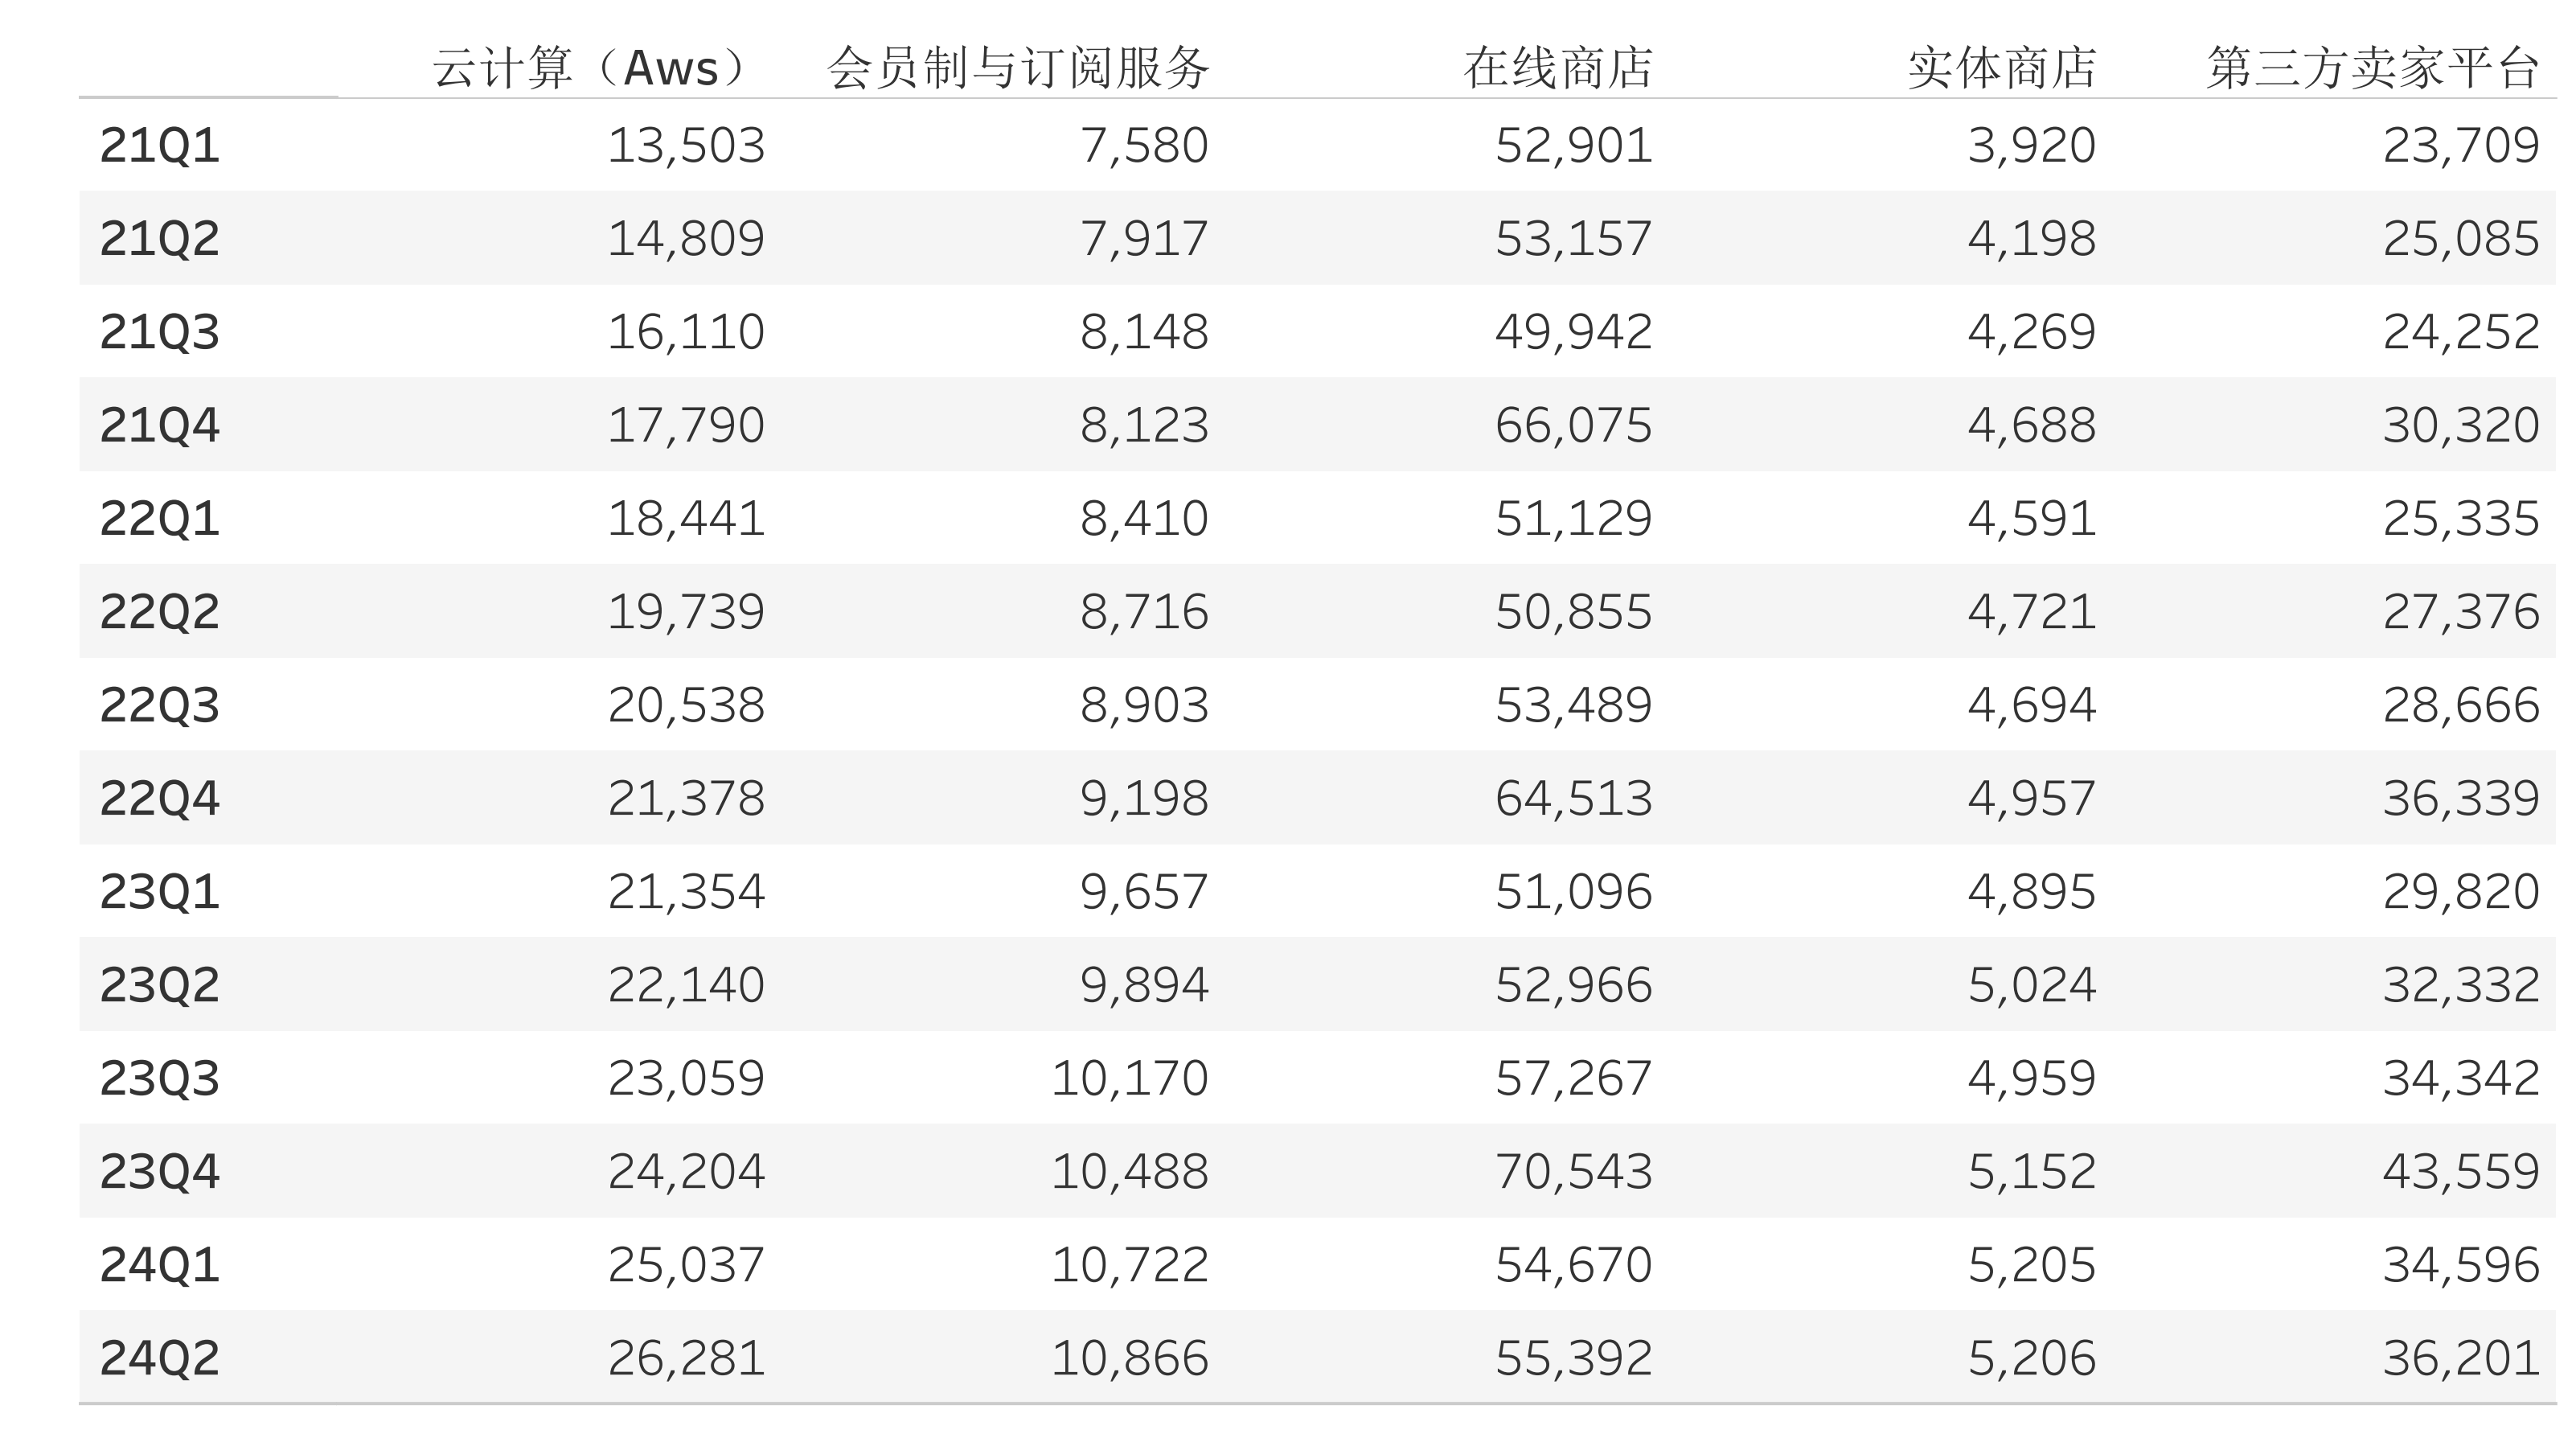
\includegraphics[width=\textwidth]{Images/Book2_00.png}
        \caption{2021年第一季度至2024年第二季度各产品组全球净收入值(单位:百万美元)}
        \label{val}
    \end{minipage}
    \begin{minipage}[t]{0.45\textwidth}
        \centering
        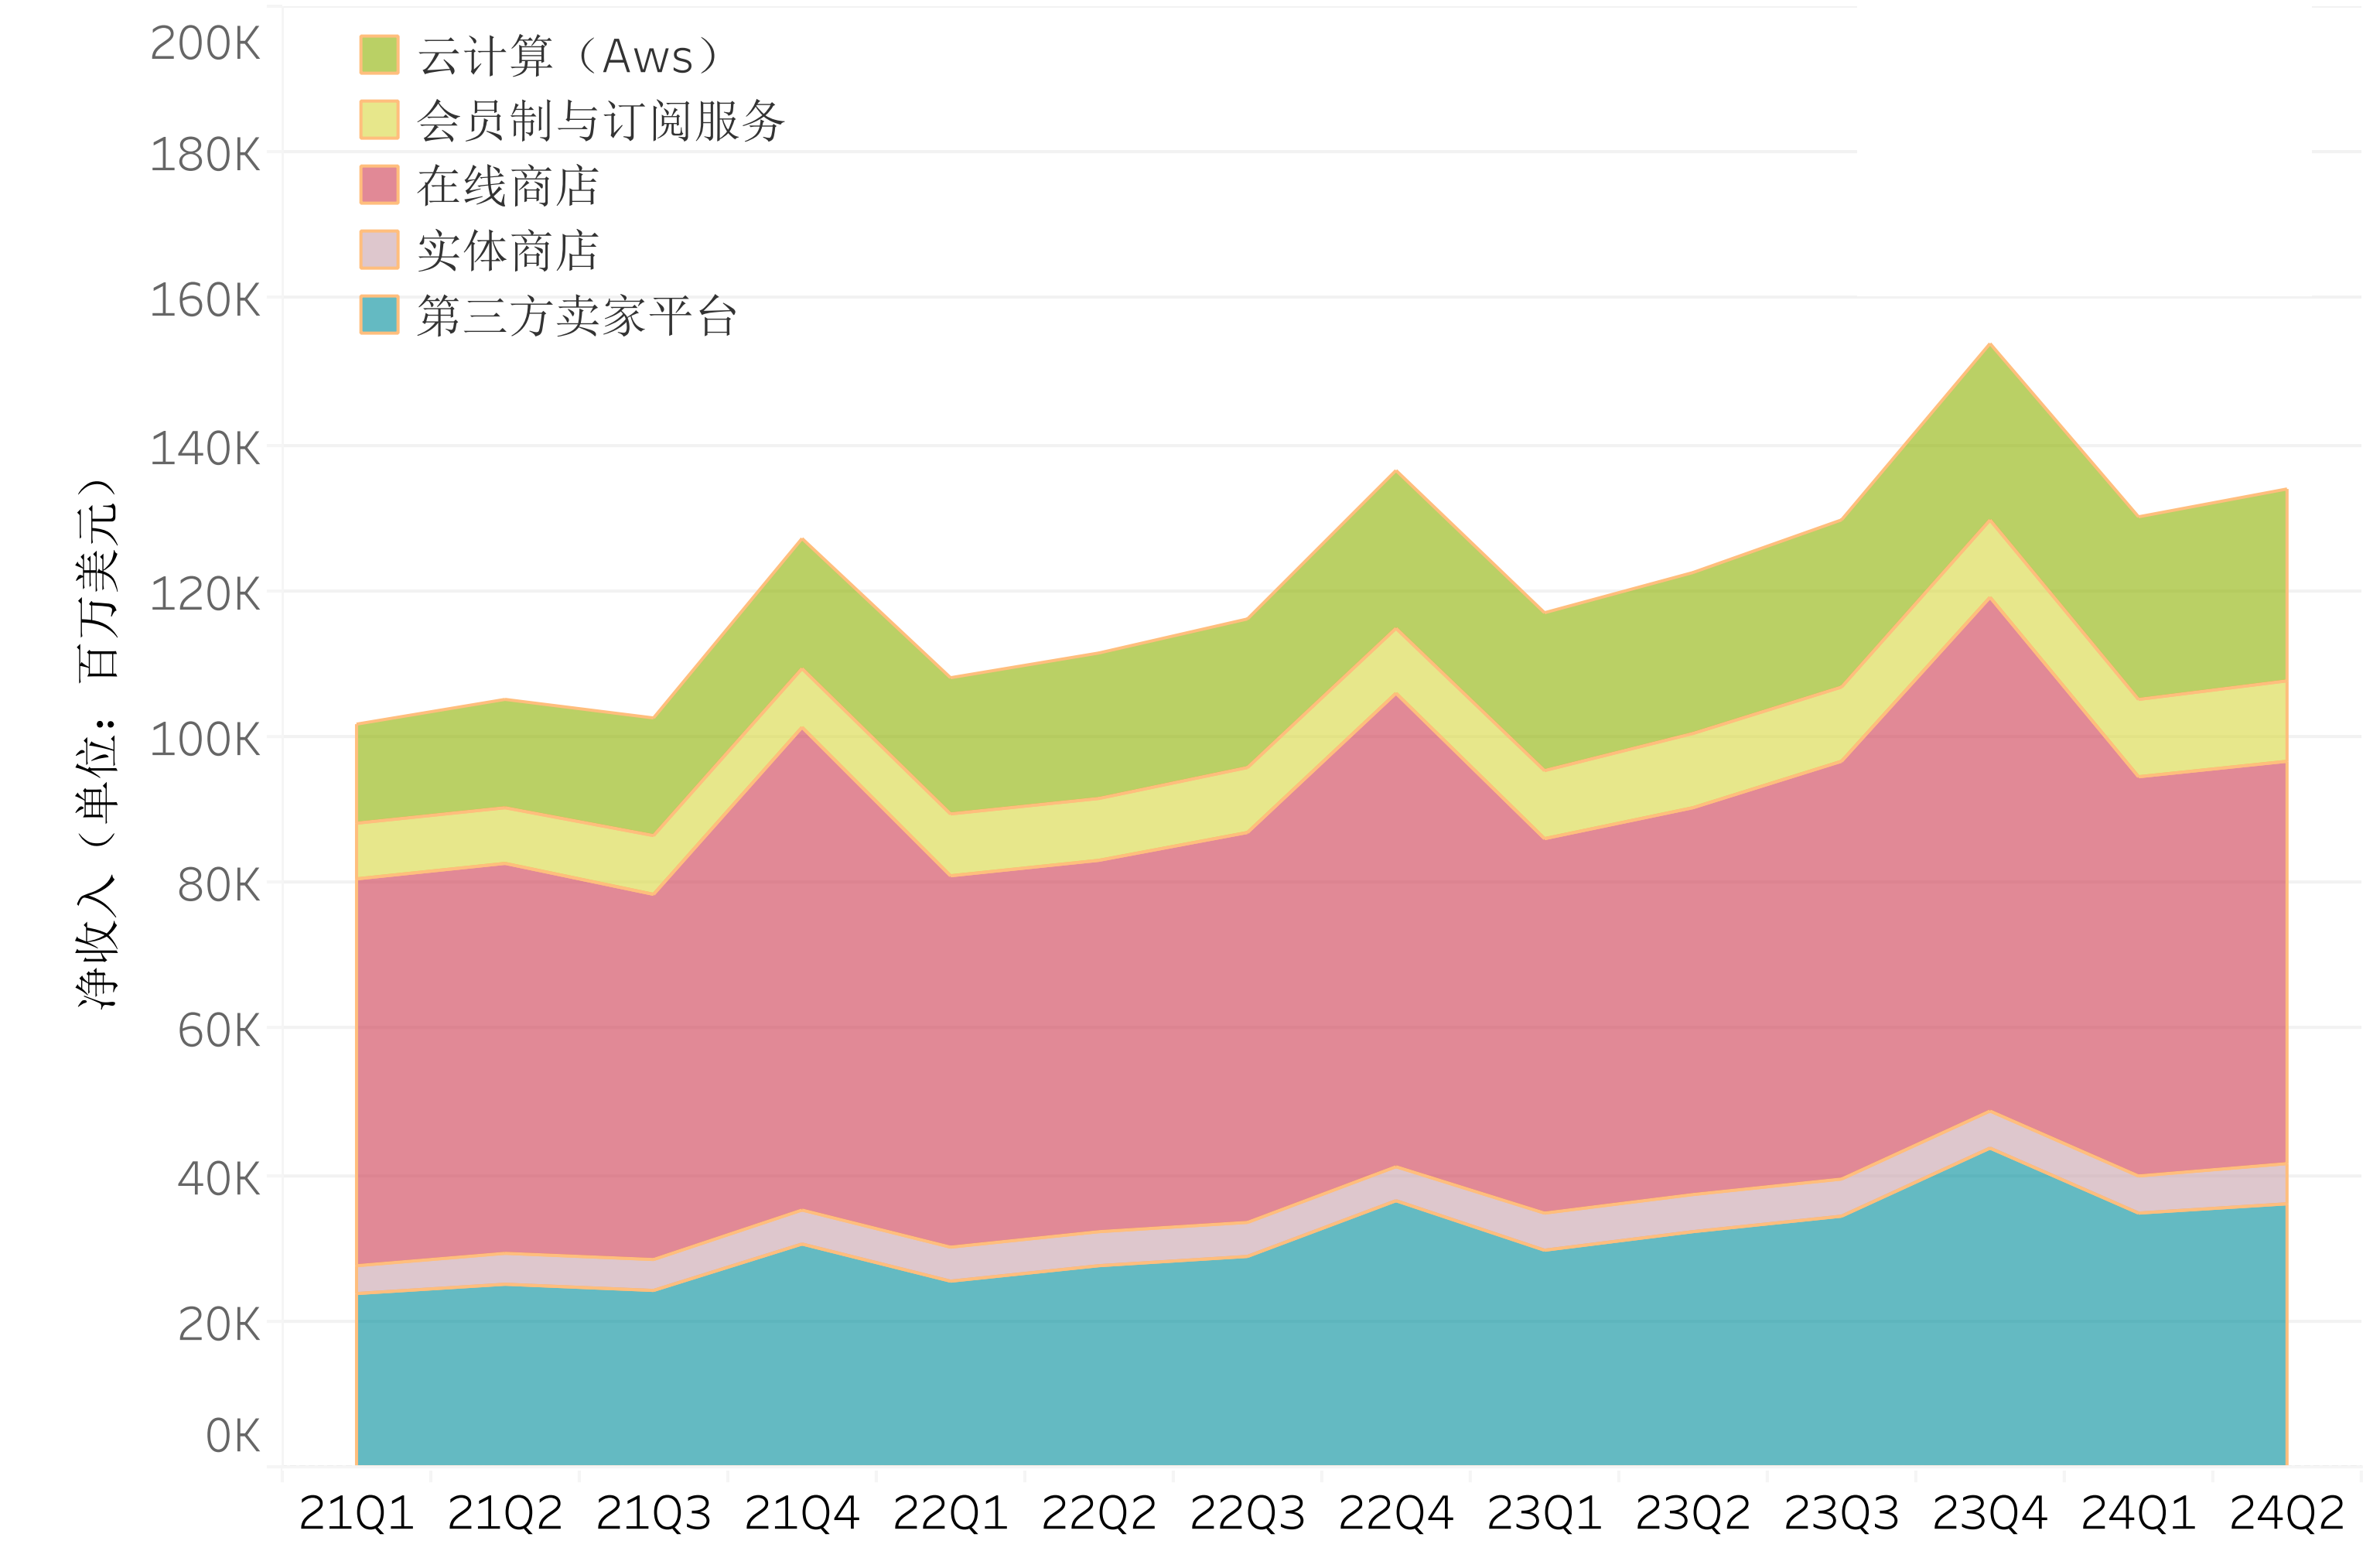
\includegraphics[width=\textwidth]{Images/Book1_00.png}
        \caption{各产品组全球净收入值变化趋势}
        \label{trd}
    \end{minipage}
\end{figure}

从图(\ref{trd})不难看出,亚马逊的全球净收入呈现季度规律性波动、但总体稳健上升的趋势,每年的第四季度都会迎来收入暴增。在2024年第二季度,在线商店仍然有最高的收益,达553.92亿美元,同时期的第二、三位分别是第三方卖家平台和云计算(AWS),实体商店则收益有限。

\begin{itemize}
    \item \textbf{在线商店(第一方)与卖家平台(第三方).} \\
    亚马逊作为零售商,可以直接采购商品并销售给消费者,也就是通常说的“自营”,图(\ref{val})可以看出,在线商店一直持续为亚马逊带来最大的收入。第三方卖家平台Amazon Marketplace也是收益的一大巨头,帮助亚马逊扩大了产品种类,它的配送方式则是Fulfillment by Amazon物流。虽然对净收入而言,第一方在线商店因其直接性获益远超第三方卖家平台,但就净销售额而言,这两个业务见的关系却是完全相反的。

    \begin{figure}[htbp!]
        \centering
        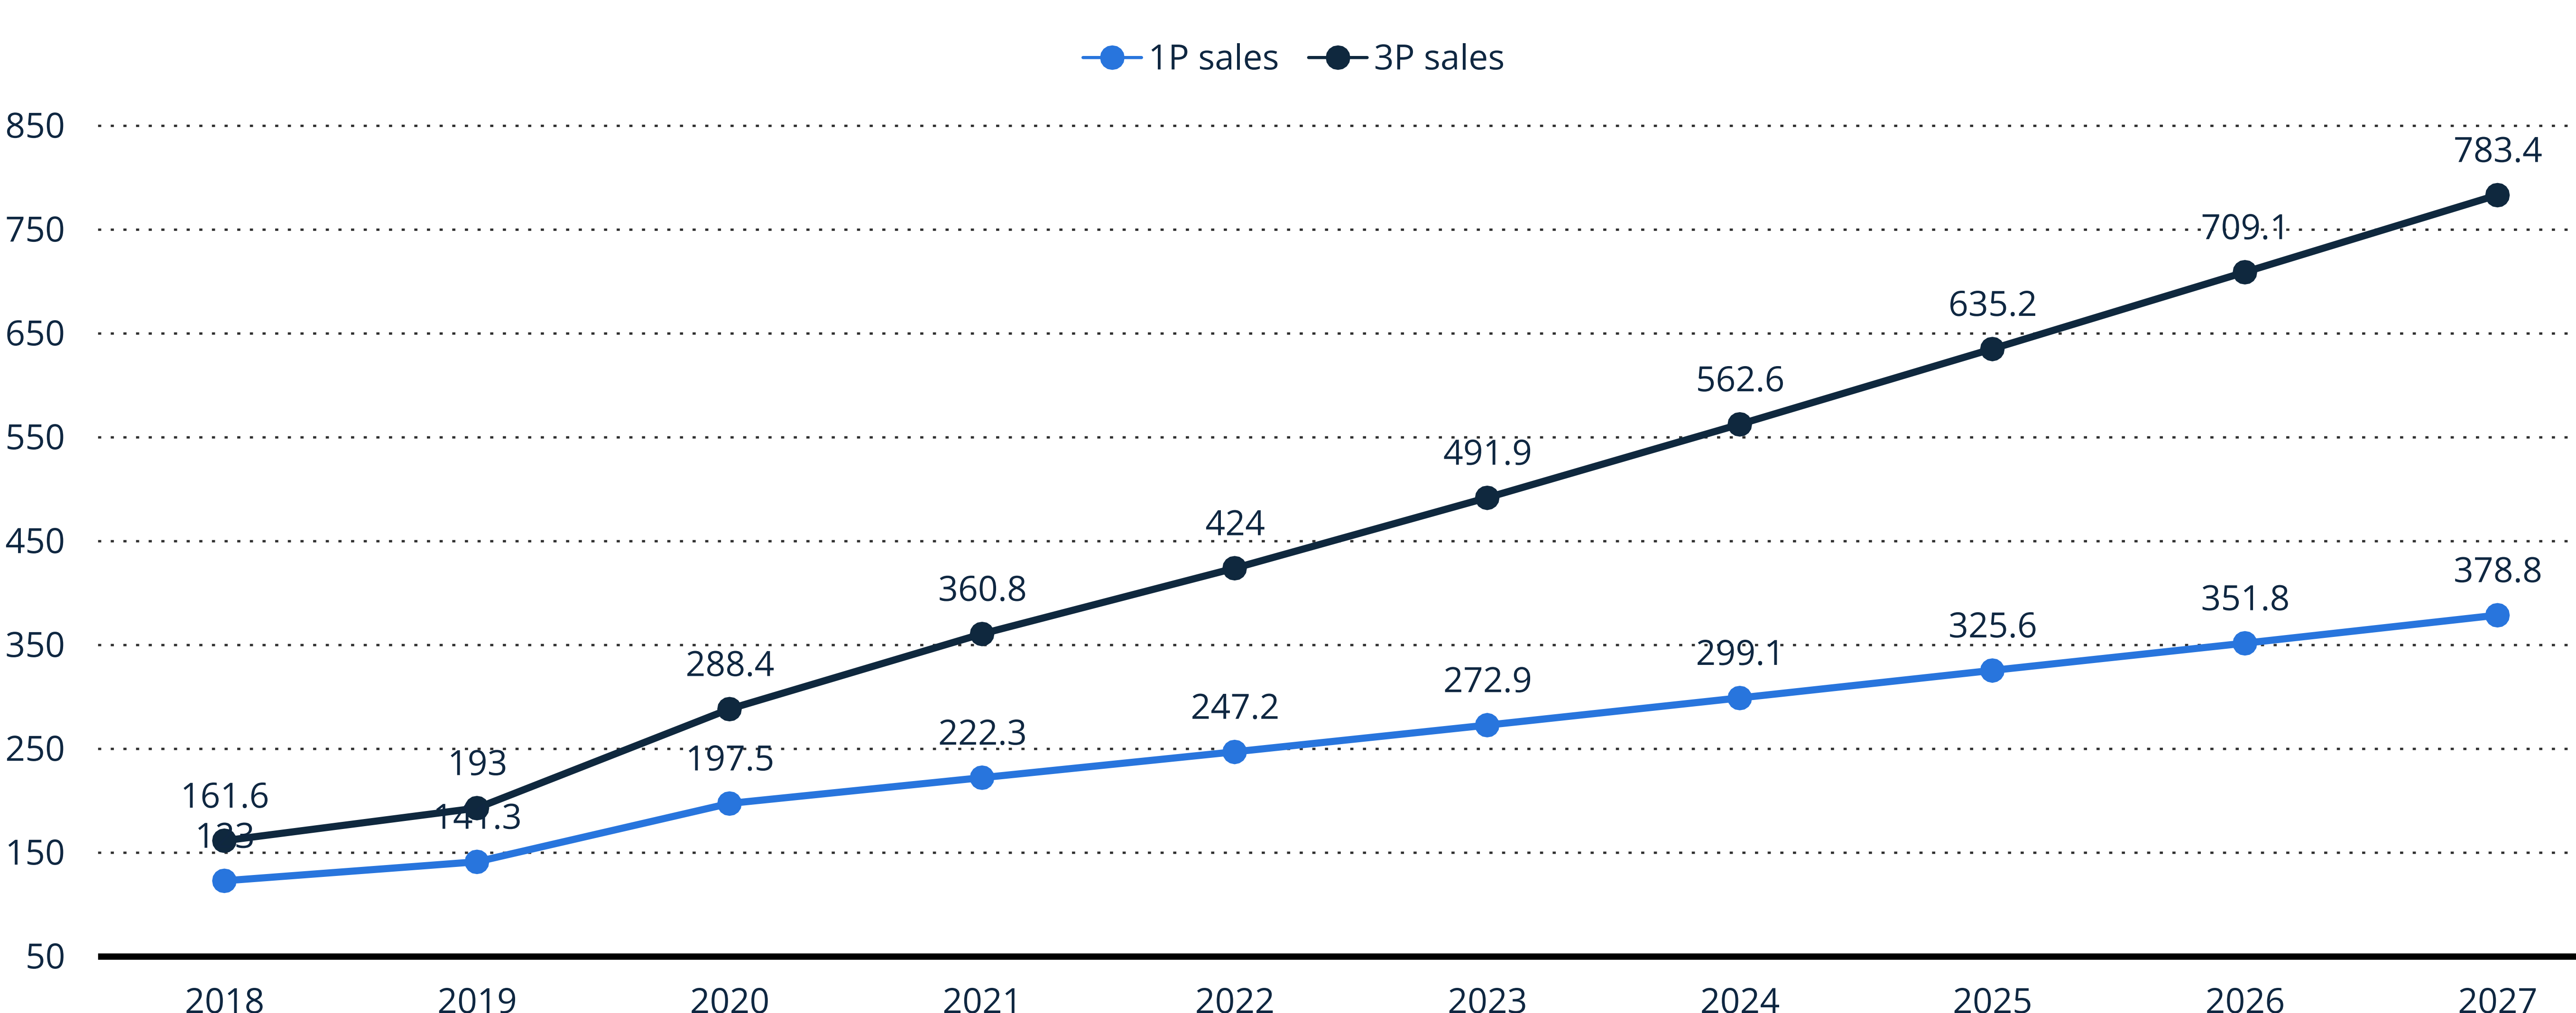
\includegraphics[width=0.95\textwidth]{Images/5.png}
        \caption{2018年至2027年(预计)第一方和第三方净销售额(单位:十亿美元)}
        \label{cut}
    \end{figure}

    从摘自Statista关于亚马逊的报告\cite{17}的图(\ref{cut}),可以推测,亚马逊作为第三方的收益率应当是远不及“自营”,但在2025年,第三方净销售额将达到第一方净销售额的接近两倍,因此从业务能力角度来看,二者则更应称之为不相上下了。
    
    \item \textbf{实体商店.} \\
    亚马逊的实体商店开设很晚,实体零售市场已经被Wlmart占据了很大一部分。虽然2017年收购Whole Foods使得Walmart、Costco和Kroger股市下跌,但这被认为是其最后一次撼动杂货商品领域\cite{18}。CEO安迪·贾西也在2022年坦言,“Amazon Fresh的扩张就像把钱冲进马桶里。”。后来Fresh商店移除“Just Walk Out”这项本想用之来成为主导的技术,亚马逊还关闭了一些商店,暂停了新店的扩张、降低价格、引入Dash智能购物车\cite{18}...最近两年的各个季度收入似乎也停滞不前(见图(\ref{rev})),对于亚马逊来说,还有很长的路要走。

    \begin{figure}[htbp!]
        \centering
        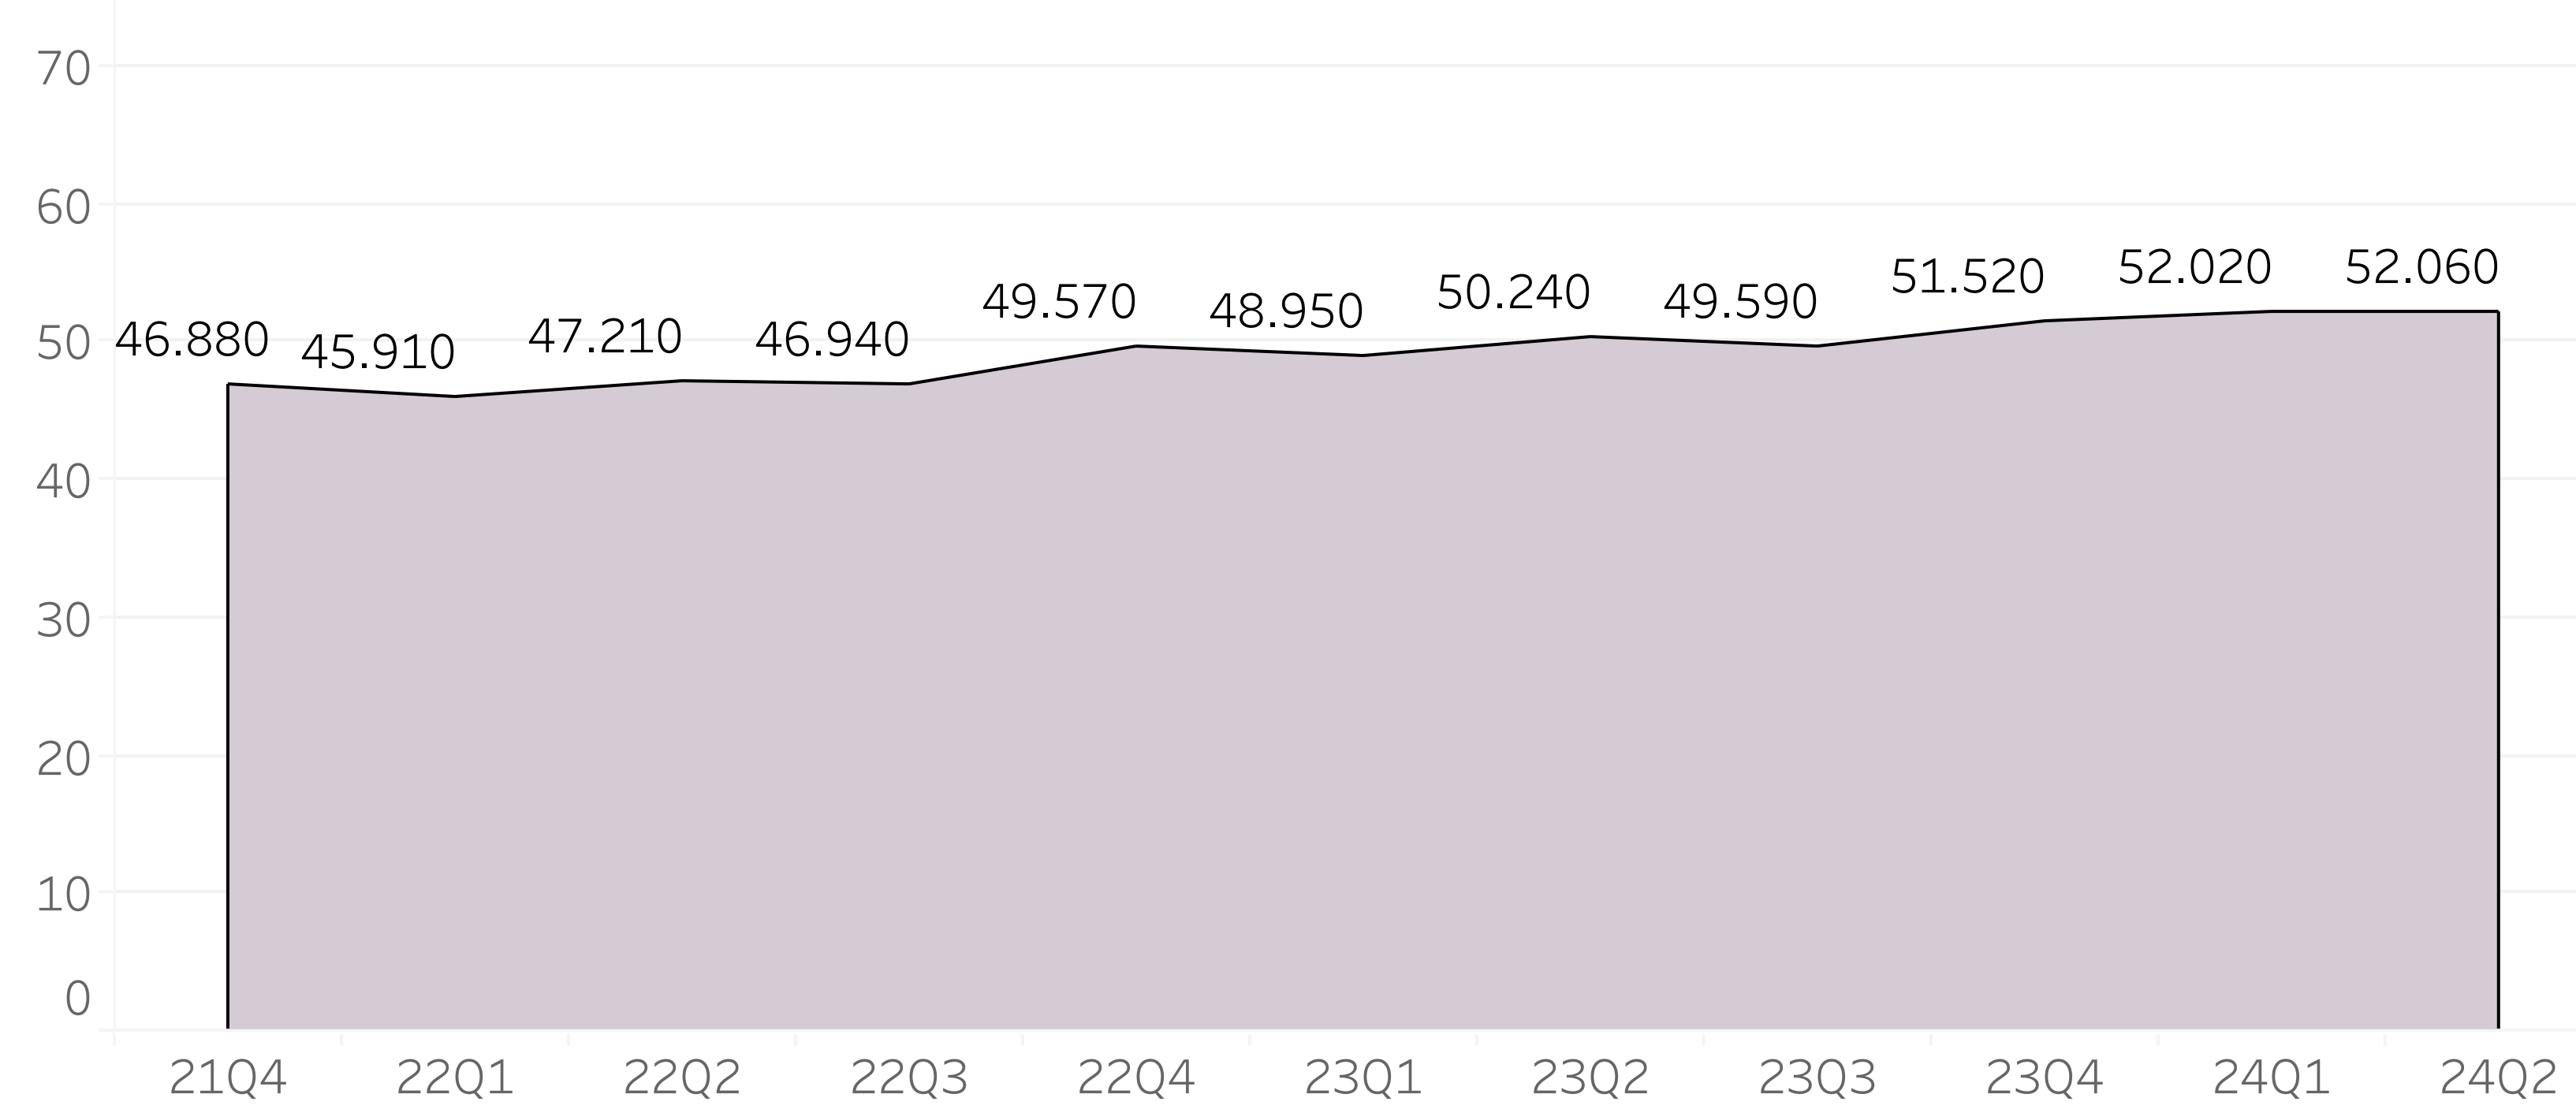
\includegraphics[width=0.8\textwidth]{Images/9.png}
        \caption{2021年至2024年各季度实体商店收入(单位:亿美元).(来源:\cite{19})}
        \label{rev}
    \end{figure}
    
    
    \item \textbf{云计算(AWS).} \\
    AWS平台提供广泛的云服务,包括基础设施即服务(IaaS)、平台即服务(PaaS)、软件即服务(SaaS)、业务流程即服务(PBaaS)以及桌面即服务(DaaS)等多种云计算解决方案,它能为用户提供计算能力、存储、数据库、分析工具、机器学习等服务来服务于个人开发者、初创企业和大企业。AWS带来的收益是巨大的,见图(\ref{fig:two_images}),SaaS作为最大的盈利方预计将在2025年取得2951亿美元的全球净营收,稍显逊色的IaaS也将创造2324亿美元的利润。
    \begin{figure}[htbp!]
        \centering
        \subfigure[]{
            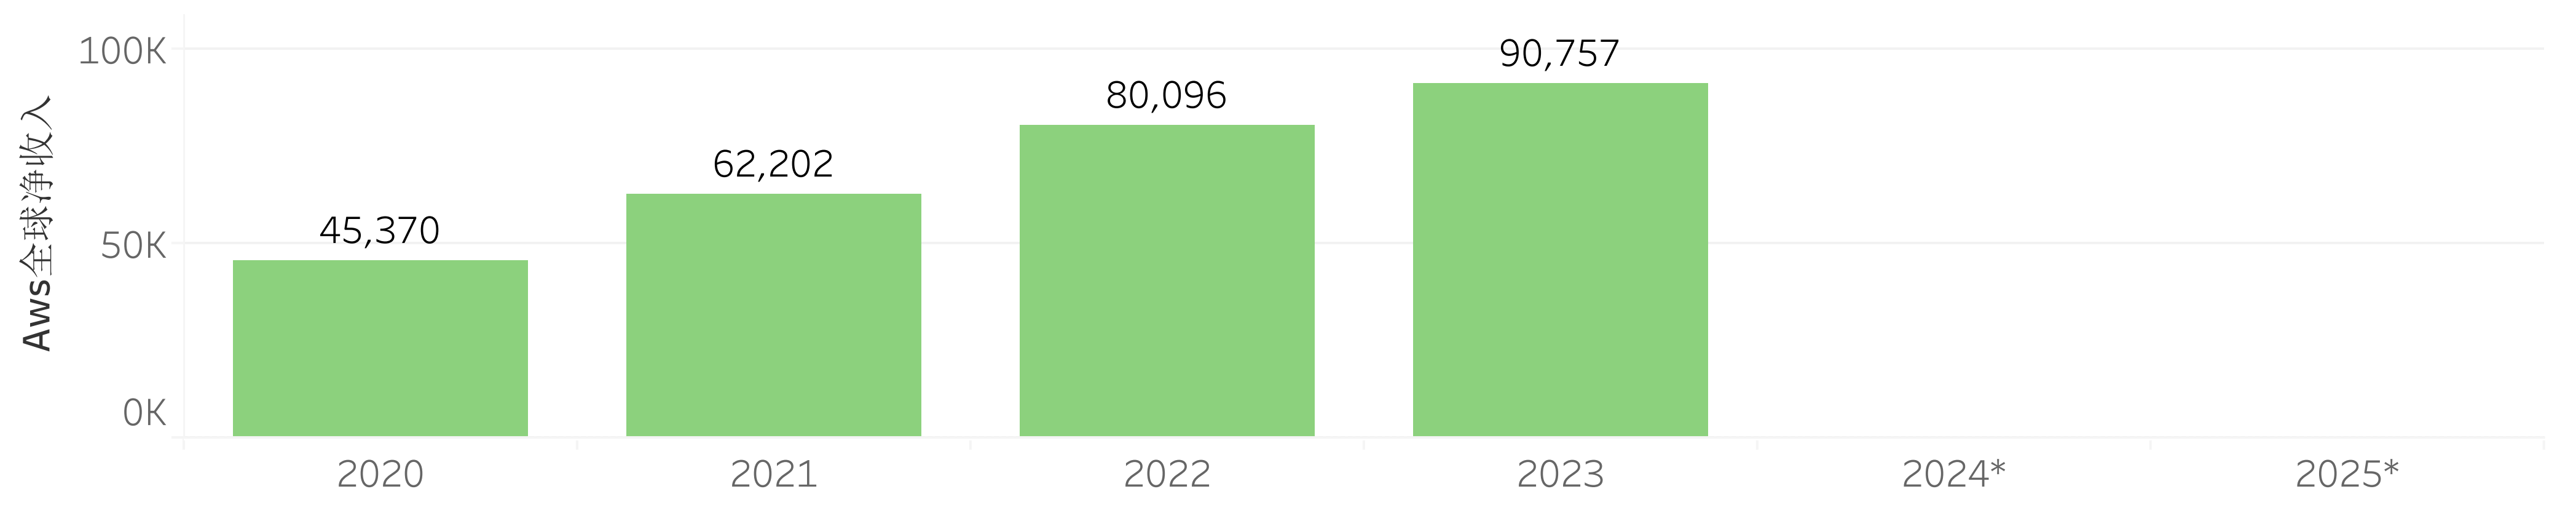
\includegraphics[width=0.85\textwidth]{Images/7.png}
        }
        \subfigure[]{
            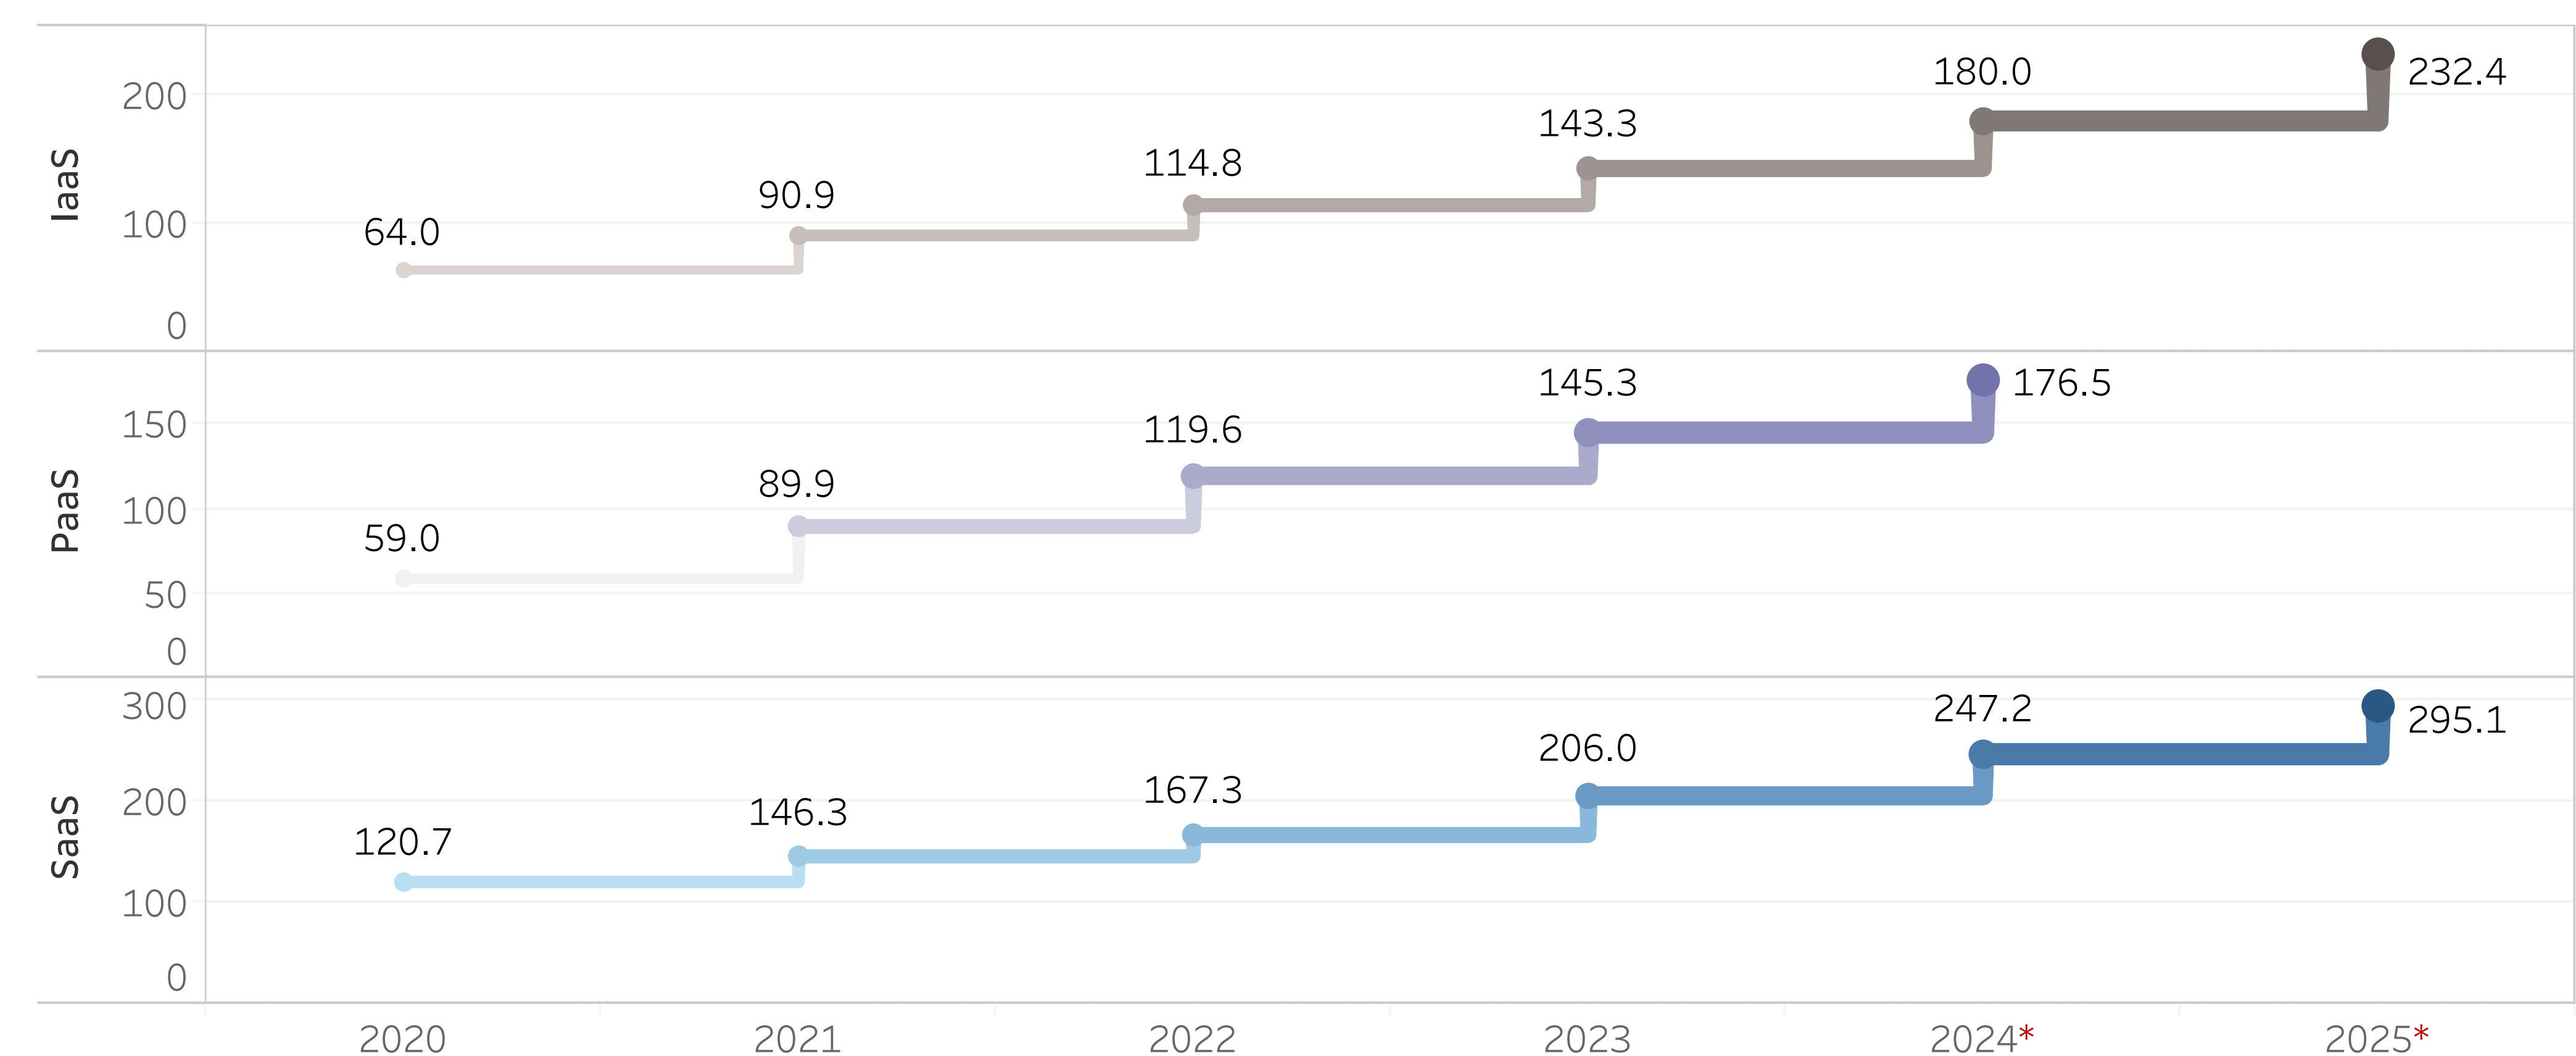
\includegraphics[width=0.85\textwidth]{Images/8.png}
        }
        \caption{(a) 2020年至2023年亚马逊全球AWS业务净营收(单位:十亿美元);(b) 2020年至2025年(预计)IaaS、PaaS、SaaS全球净营收(单位:十亿美元).(来源:\cite{20})}
        \label{fig:two_images}
    \end{figure}
    
    
    \item \textbf{会员制与订阅服务.} \\
    2005年2月,亚马逊推出了“Amazon Prime”服务,并在后来成为其最知名、最赚钱的服务之一。这项服务每年收取会员79美元并提供无限制的两天送货,在最开始五年,网上购物这一概念并不为大众所熟悉,但经过服务扩张(如引入视频订阅等),服务订阅数大幅增长。根据Search Logistics提供的数据,从2013年到2021年,亚马逊的净销售额增长了约290亿美元,这很大程度得“归功”于COVID-19,在那三年,“Amazon Prime”的订阅用户直接增加了约2800万,用户总数预测将在2025年达到1.683亿\cite{13}。

    \begin{figure}[htbp!]
        \centering
        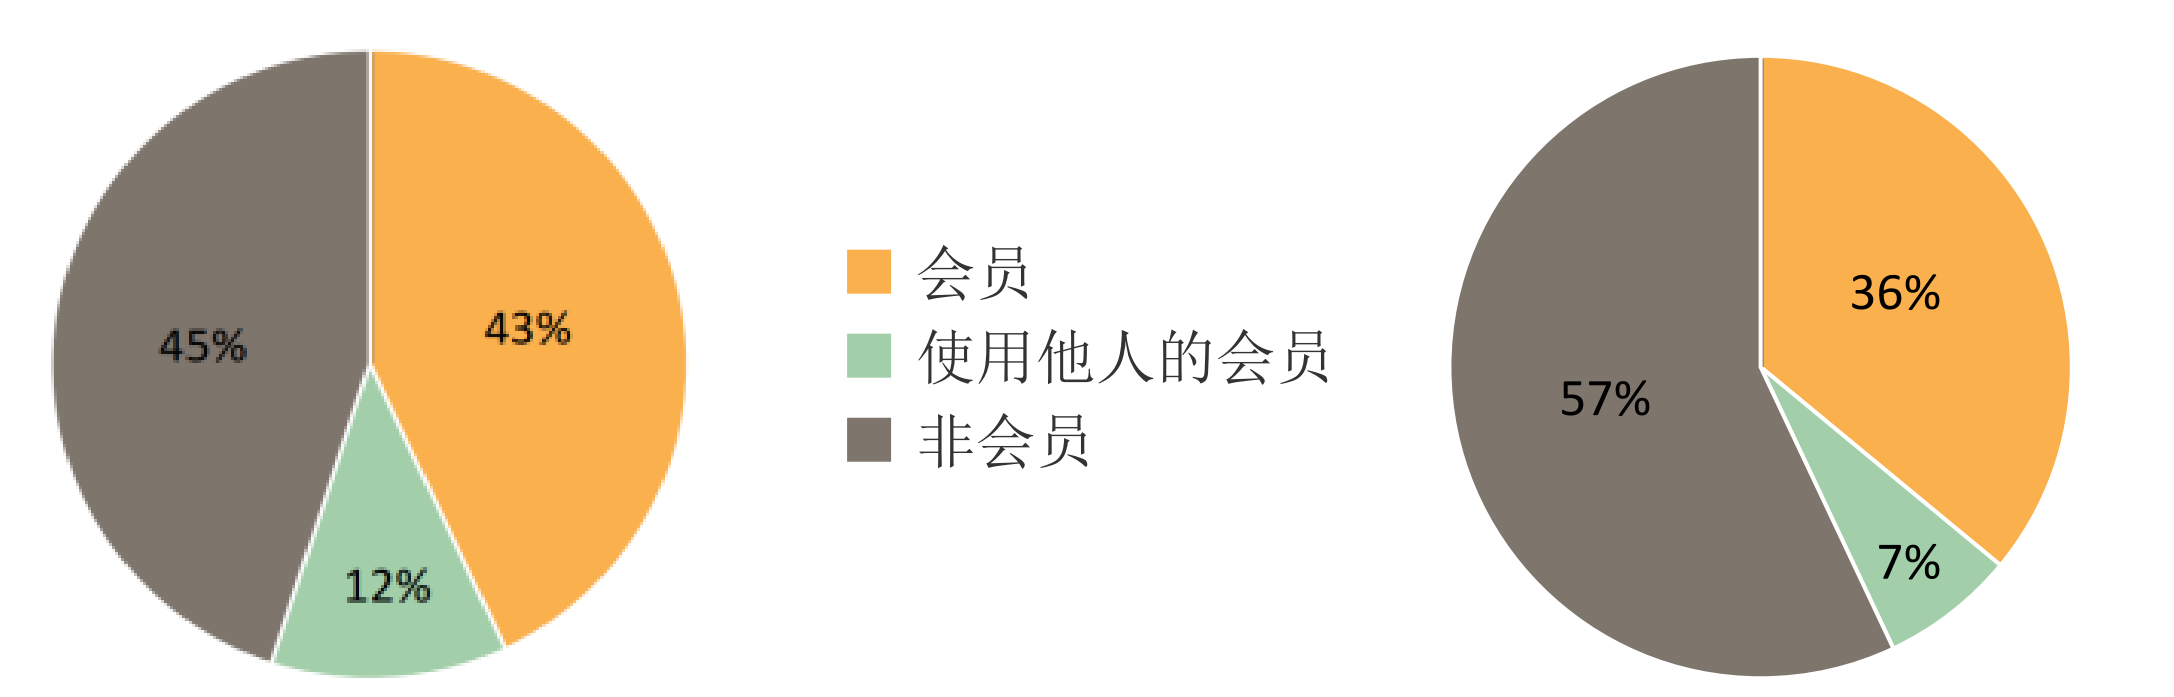
\includegraphics[width=0.75\textwidth]{Images/6.png}
        \caption{拥有会员的购物者比例(左:加拿大-2022年1月统计;右:澳大利亚-2023年2月统计).(来源:\cite{16})}
        \label{perc}
    \end{figure}

    如果考虑整个用户群体,那么图(\ref{perc})中显示的亚马逊会员的占比则十分高,且这个优势在更多国家也有体现——如在一项2023年1月的调查中,日本地区当前在订会员占比44.49\%,还有11.94\%的人曾经订购过会员;2021年,西班牙地区仅仅有超过一半的人订购会员,但到了2023年,这一比例则达到了71\% \cite{16}。订阅服务本身不但带来了利润收入,也促进了消费行为,2021年的研究就发现一名“Amazon Prime”会员每年通过亚马逊的平均消费比非会员提高约133.3\% \cite{13}。
    
\end{itemize}

\subsection{其他业务}
除以上五个业务外,亚马逊还有如Amazon Business(针对B2B贸易市场)、Amazon Studios和Amazon Music(电影与音乐制作)、Amazon Air(物流服务)等业务,此外,亚马逊也在逐步进入金融领域,提供包括Amazon Pay和Amazon信用卡等在内的多种支付和金融服务。

亚马逊通过不断扩展和多元化其业务,从传统的电商巨头逐步发展成为科技、娱乐、金融、硬件等多个行业的综合性跨国公司。这种多元化的布局不仅增强了其抗风险能力,也为未来的增长开辟了更多潜力。综合来看,亚马逊将长期在全球市场上保持竞争优势和持续增长的动力。

\subsection{整体业务结构与商业模式深析}
亚马逊的五大业务是相辅相成的,它们的协同效应使得亚马逊能够通过整合资源,形成一个高度互补、相互促进的生态系统。一篇在今年2月发布于FourWeekMBA的报告中就清晰地绘制了它们之间的关系,见图(\ref{rela})。

\begin{figure}[htbp!]
    \centering
    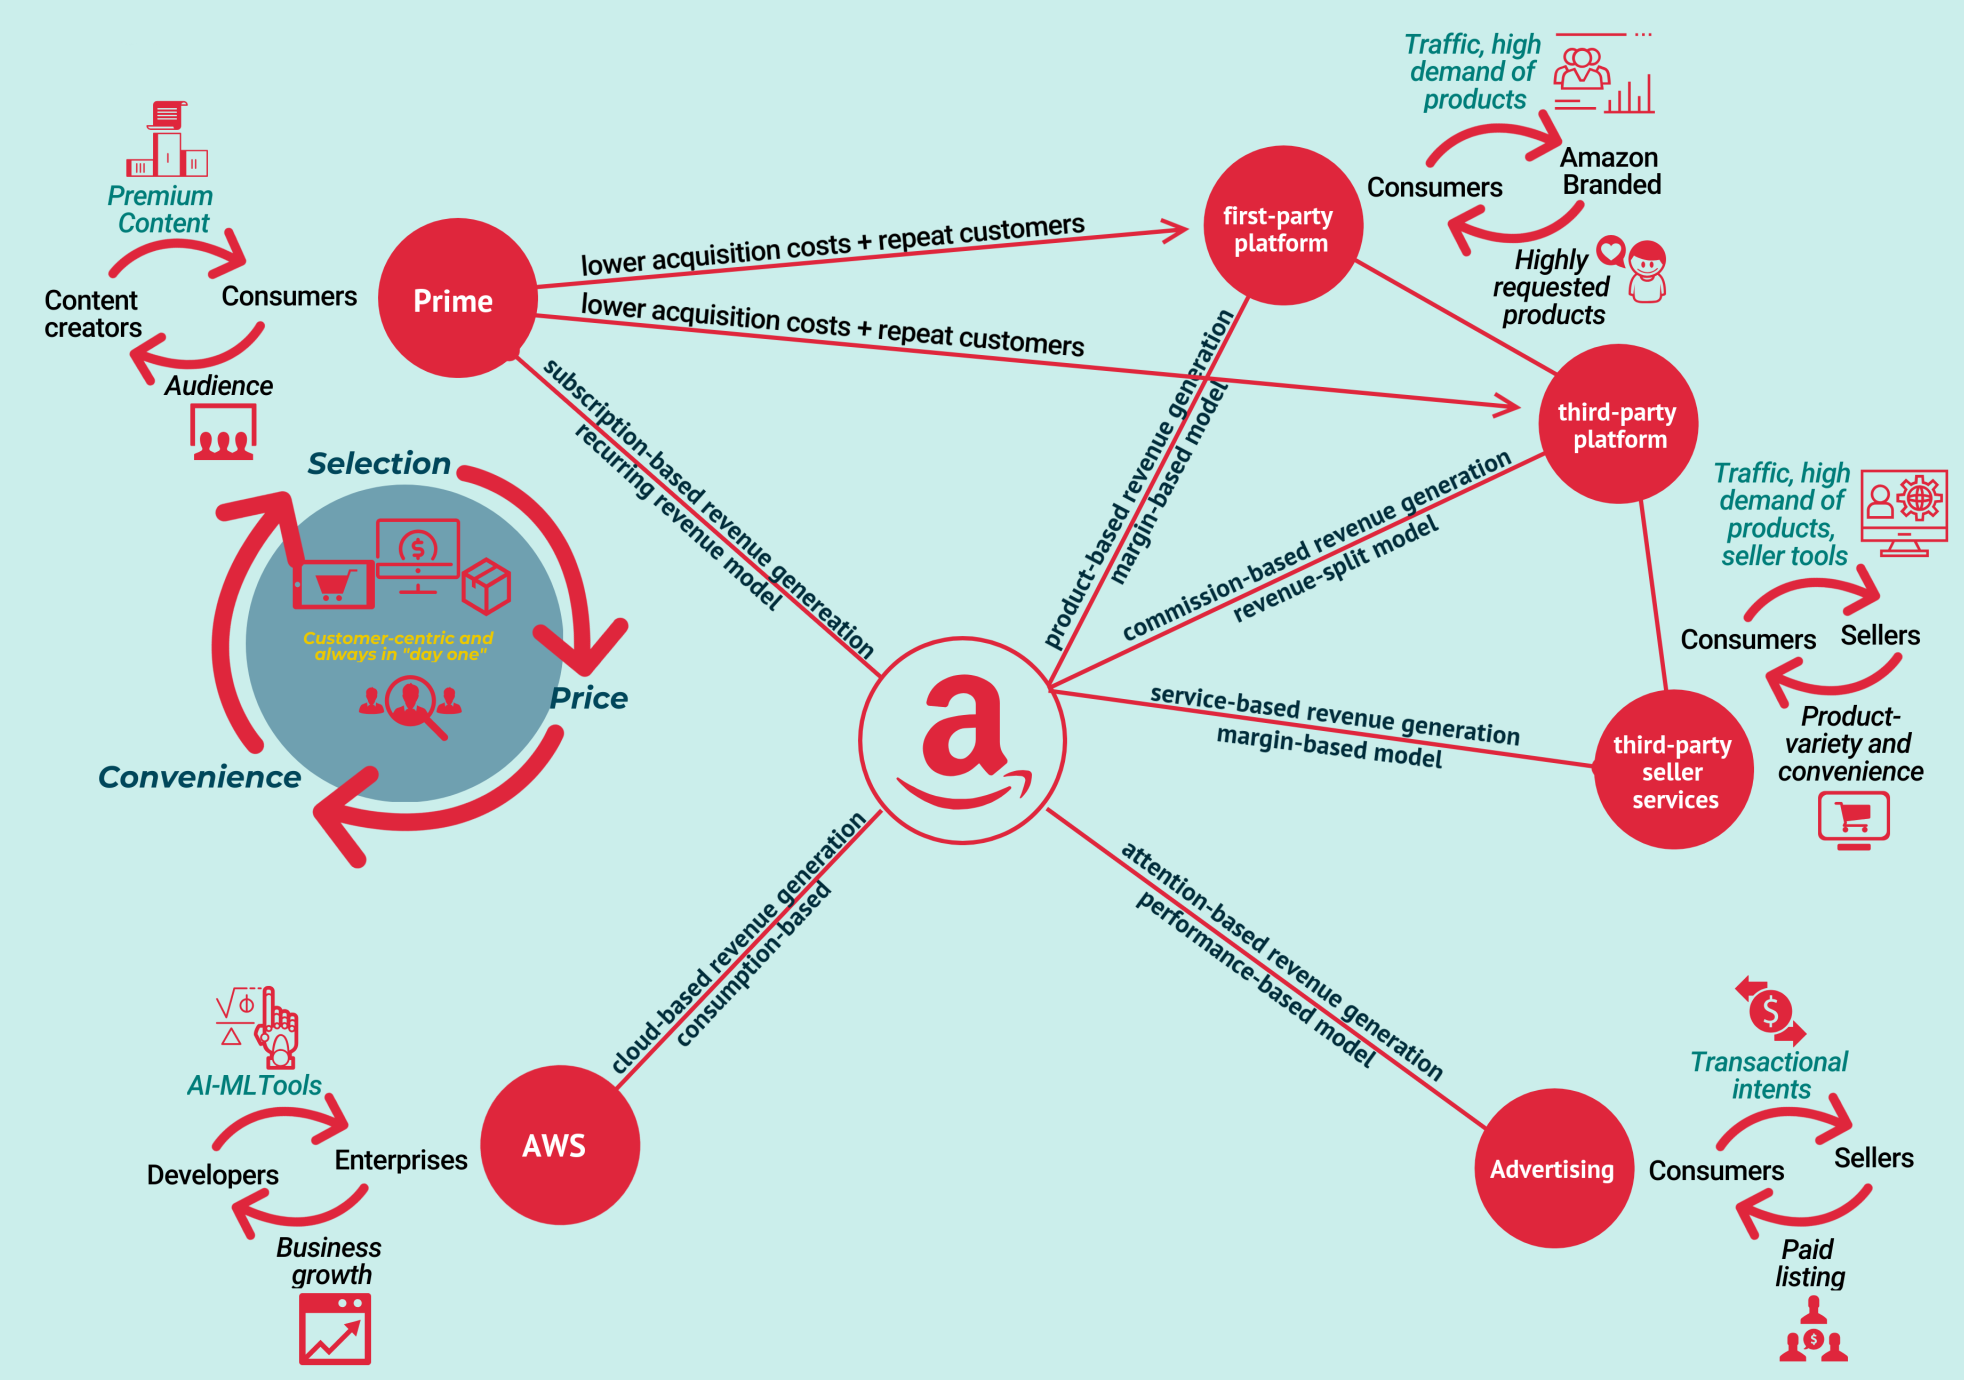
\includegraphics[width=0.8\textwidth]{Images/amazon-value-proposition-1.png}
    \caption{亚马逊主要业务间的价值促进关系.(来源:\cite{23})}
    \label{rela}
 \end{figure}

很容易看出,亚马逊的收益可以被概括为三大类:基于关注度、基于技术、基于产品,其中第一项含订阅收益(也就是Prime)和广告收益;第二项就是AWS带来的收益;第三项是产品的直接(也就是第一方)、间接(也就是第三方)售卖收益。

不妨从关注度看起,广告使消费者对卖家商品产生兴趣,卖家为了吸引消费者就会投放广告,若投放的广告为“Amazon Prime”服务,那么就直接推动了订阅收益的增加。与此同时,订阅服务会根据购物行为偏好向消费者不断推送个性化信息,以此刺激消费者在第一方、第三方平台消费的欲望,且这批订阅用户也成为了消费平台上的“熟面孔”。第一方平台与第三方平台有互补效应,第一方平台专注于高质、高量产品,而第三方平台则提供了一个更加广泛的选择空间,它们又同时依托于亚马逊的物流、供应链系统,以此收益。AWS业务其实是一个比较特殊的存在,虽然图(\ref{rela})中它并没有与其他业务关联,但本质上其无处不在,或者在某种意义上可以说是支撑整个生态系统正常运行的“生命水晶”。AWS系统允许开发者使用AI或机器学习工具,将开发的模型提供给企业应用,以此带来商业效益增幅,这里的模型可以是个性化推荐模型、大数据订阅推荐算法、商品定价模型等等,实际上AWS使得更多优秀的开发者们得以满足企业需要,也作为一种不可或缺的“介质”使得收益源源不断涌向了亚马逊。

这张关系网络没有谈及的一个业务是线下商店。线下商店因为其特殊存在形式,虽然并不是与其他业务都毫无关系,但是相较于其他四者,它的存在感自然不高。亚马逊的线下商店与其在线业务相互促进,形成了一个无缝的全渠道购物体验,如实体店Amazon Go、Amazon Fresh和Whole Foods允许“线上下单,线下取货”,并且提供便利的退货服务等,以此来提升用户黏性(也就可以称之为基于关注度的收益)。尽管亚马逊关闭了一些像Amazon Books和4-Star未能产生显著收入的实体店,但它们仍成为了提升企业竞争力和适用面的一环\cite{26}。

再谈谈亚马逊的商业模式,在报告\cite{32}中有整体概览和一些解读,图(\ref{rela})中有更为细致的分类:(1)“Value Model” - 亚马逊的使命是“通过线上和实体店为消费者服务,注重选择、价格和便利”,这就是其作为平台的根本价值;(2)“Technological Model” - 双边网络效应,加入亚马逊第三方卖家服务的卖家越多,可供选择的产品种类就越多,价格也越合理。这反过来又会吸引越来越多在亚马逊购物的用户,出色的用户体验也会产生回头客(这也就是图(\ref{rela})中的“performance-based model”),从而促使其他人加入;(3)“Distribution Model” - 增长建立在其多年来打造的强大品牌之上,其引擎是由核心技术平台、价格合理的多样化产品以及坚实的基础平台构成的;(4)“Financial Model” - 通过积极的现金转换周期产生现金流(就是图(\ref{rela})中的“recurring revenue model”),可以投资于其运营。库存可以快速转化为现金,供应商或第三方商店则可以在 30-60 天内收到付款。图(\ref{rela})中还提到的商业模式有“consumption-based model”(也就是按需付费,客户只为他们使用的计算能力、存储或网络资源付费,而不需要预先购买或长期订阅,十分灵活)、“margin-based model”(也就是产品或服务销售时获取的利润差,因此注重优化供应链、降低成本和大规模销售)、“revenue-split model”(意为亚马逊和卖家共享销售收入,每笔销售将以一定比例收取佣金)。

关于亚马逊的五大业务,第一方在线商店的模式为“margin-based”,第三方卖家平台的模式为“revenue-split”,实体商店的模式为“recurring revenue”和“performance-based”、AWS的模式为“consumption-based”、“Prime”会员制的模式为“recurring revenue”和“performance-based”。

以下就第一方在线商店和第三方卖家平台的“margin-based”盈利模式和 AWS “consumption-based”的定价策略分别深入分析。
\begin{itemize}
    \item \textbf{第一方在线商店和第三方卖家平台的“margin-based”盈利模式.} \\
    在第一方在线商店中,品牌通过亚马逊的Vendor Central平台将产品以批发价卖给亚马逊,亚马逊再以自己的定价出售这些产品。亚马逊作为“零售商”直接向消费者销售,产品标记为“亚马逊销售和发货”,其利润空间相对较小,利润率通常在8\%至15\%之间\cite{33}。

    在第三方卖家平台中,卖家通过亚马逊的Seller Central平台自行销售产品,卖家可以自己定价和管理库存,亚马逊为其提供销售平台、快递运送等,通过收取各种费用从中获利。其中一个为Referral Fee(推荐费),通常是商品销售价格的10\%至17\%不等(来自2024年1月更新的规定\cite{34}),视品类而定(如电子产品的费率更低);还有一种为Fulfillment Fees(履约费),如果第三方卖家选择使用亚马逊的FBA服务,那么就需要支付仓储、配送、管理、退货的费用,这与商品的大小和重量有关,不过如果该产品在Ships in Product Packaging (SIPP) program中,那么折扣后的价格为0.04至1.32美元不等\cite{34}。
    
    \item \textbf{AWS 的“consumption-based”定价策略.} \cite{36}
    \begin{enumerate}
        \item \textbf{On-Demand.} \\
        这种方案允许用户按小时(取决于类型)支付计算容量费用,无需长期承诺或预付款。此模型提供了最高的灵活性,使用户可以随意启动和停止运行,这对于具有短期、不规则或不可预测的工作负载且无法中断的程序来说是理想的选择,它也是正在尝试AWS的新用户的首选。当然,它的价格就相对其他更高一些,假设在美国东部地区运行一个t3.medium实例(中型虚拟机),那么每小时费用约为0.0376美元。
        
        \item \textbf{Spot Instances.} \\
        这种方案允许用户以与按需价格相比大幅折扣的价格购买未使用的 AWS 容量。与按需实例相比,竞价实例可节省高达 90\% 的成本,因此对于注重成本且工作负载灵活的用户来说,竞价实例是一个有吸引力的选择。仍然以t3.medium为例,每小时的价格甚至可以低至0.015美元。不过如果 AWS 需要收回容量,只需提前两分钟通知即可终止,因此它则更适用于可容忍中断的非重要任务。
        
        \item \textbf{Reserved Instances.} \\
        这种方案预提供了更大幅得折扣(最高可达 75\%),但前提是承诺在特定区域使用特定实例类型一至三年,因此该方案非常适合使用情况稳定或可预测的关键程序,这些应用程序可以承诺长期使用一定水平的 AWS 资源,而这个方案也能使用户使用更加安心,价格则相较于Spot Instances更高一些。还是以一个t3.medium为例,其一年期的预付款费用约为265美元,按小时计算大约0.0303美元;三年的预付款费用约为639美元,按小时计算则大约0.0073美元。
        
        \item \textbf{Saving Plans.} \\
        这种方案与Reserved Instances相比则是更灵活,用户在承诺一年或三年内保持一致的使用量后,可在任何 AWS 服务上节省高达 72\% 的指定使用量,且可以在任何实例类型、大小甚至 AWS 服务之间切换,此方案则更加适配不断变化的技术和应用需求。对于t3.medium来说,一年期承诺只需0.028美元每小时,三年期承诺也只需0.020美元每小时。
        
        \item \textbf{Dedicated Hosts.} \\
        专有主机是具有 AWS EC2 实例容量的物理服务器,完全专用于用户帐户。此选项对于禁止与其他租户共享服务器的监管要求或需要特定服务器的许可非常有用。专用主机提供对实例在物理服务器上放置位置的可见性和控制,帮助用户满足合规性和监管要求,由于其“专有”的特点,它自然也是最昂贵的选择了。t3.medium的专用主机费用约为 0.21美元每小时,不过这个价格也包括了整台物理服务器的费用。
        
    \end{enumerate}  
    
\end{itemize}
 AWS主要有以上五种定价方案,在\cite{36}中它们进行了探讨,而EC2则还有一种定价方式。
 
    \begin{figure}[htbp!]
        \centering
        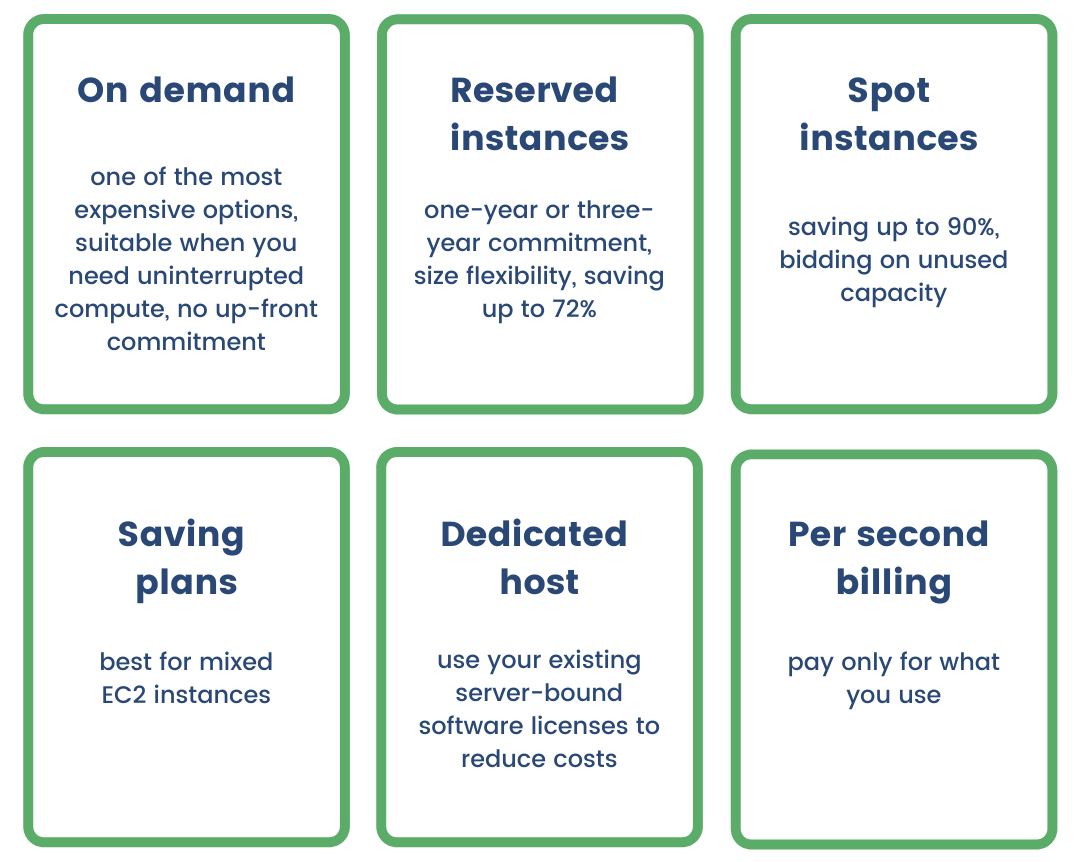
\includegraphics[width=0.7\textwidth]{Images/1618012212696.png}
        \caption{亚马逊AWS EC2的六种定价策略.(来源:\cite{35})}
        \label{fiv}
     \end{figure}
     
(6)\textbf{Per-Second Billing}可以看作是On-Demand的一种变种方案,在这里计费最小单位变成了60秒,十分适用于短时间运行的任务。


\newpage
\newgeometry{right=1in,left=1in,top=1in,bottom=0.75in}
\addcontentsline{toc}{section}{参考文献}
\begin{thebibliography}{99}

    \bibitem{1} Statista. (n.d.). \textit{B2B eCommerce - In-depth Market Insights \& Data Analysis}. Statista. \\ Retrieved September 6, 2024, from https://www.statista.com/study/44442/in-depth-report-b2b-e-commerce/
    
    \bibitem{2} eMarketer. (June 1, 2023). Retail e-commerce sales worldwide from 2014 to 2027 (in billion U.S. dollars) [Graph]. In \textit{Statista}. \\ Retrieved September 06, 2024, from https://www.statista.com/statistics/379046/worldwide-retail-e-commerce-sales/

    \bibitem{3} Goti, A., Querejeta-Lomas, L., Almeida, A., de la Puerta, J. G., \& López-de-Ipiña, D. (2023). Artificial Intelligence in Business-to-Customer Fashion Retail: A Literature Review. \textit{Mathematics, 11}(13), 2943. doi:10.3390/math11132943.

    \bibitem{4} Statista Digital Market Insights. (May 15, 2024). Retail e-commerce revenue worldwide from 2019 to 2029, by segment (in trillion U.S. dollars) [Graph]. In \textit{Statista}. \\ Retrieved September 08, 2024, from https://www.statista.com/forecasts/1223973/e-commerce-revenue-worldwide-by-segment

    \bibitem{5} Statista. (n.d.). \textit{C2C e-commerce}. Statista. \\ Retrieved September 8, 2024, from https://www.statista.com/study/123971/c2c-e-commerce/

    \bibitem{6} Statista. (n.d.). \textit{Cross-border e-commerce}. Statista. \\ Retrieved September 8, 2024, from https://www.statista.com/study/85361/cross-border-e-commerce/

    \bibitem{7} AstuteAnalytica India Pvt. Ltd. (2024, March 14). Global Cross-Border E-Commerce Market to Hit Revenue of USD 16,454.9 billion by 2032 | 3\% of US/Canada E-commerce Revenue is International, Says Astute Analytica. \textit{Yahoo Finance}. \\ Retrieved September 8, 2024, from https://finance.yahoo.com/news/global-cross-border-e-commerce-143000804.html

    \bibitem{8} 李嘉雯. (2024). 跨境电商的发展现状与前景研究. \textit{全国流通经济}(07), 60-63. \\ doi:10.16834/j.cnki.issn1009-5292.2024.07.034.

    \bibitem{9}  Facts and Factors. (2023, January 30). \textit{Cross-border B2C e-commerce market size \& share analysis report 2022-2030}. \\ Retrieved September 8, 2024, from https://www.fnfresearch.com/cross-border-b2c  \\  -e-commerce-market

    \bibitem{10} 上海社会科学院, 渣打银行, 理财周刊, \& Dun \& Bradstreet. (2023, November 7). \textit{2023跨境电子商务发展报告}.

    \bibitem{11} Alibaba. (2024, July 18). \textit{The top 11 Amazon competitors (2024)}. Alibaba. \\ Retrieved September 9, 2024, from https://seller.alibaba.com/businessblogs/the-top-11-amazon-competitors-2024-px002b9rk

    \bibitem{12} Your Ecom Agent. (n.d.). \textit{Walmart vs Amazon vs Alibaba: A comparative analysis of e-commerce giants}. Your Ecom Agent. \\ Retrieved September 9, 2024, from https://www.yourecomagent.com/amazon-and-alibaba/ \\ walmart-vs-amazon-vs-alibaba-a-comparative-analysis-of-e-commerce-giants/

    \bibitem{13} Hopkins, C. (2023, May 1). \textit{The History of Amazon and its Rise to Success}. \\ Retrieved September 9, 2024, from https://sites.lsa.umich.edu/mje/2023/05/01/the-history-of-amazon-and-its-rise-to-success/

    \bibitem{14} Zippia. (n.d.). \textit{Amazon company history timeline}. Zippia. \\ Retrieved September 9, 2024, from https://www.zippia.com/amazon-careers-487/history/
    
    \bibitem{15} Wikipedia contributors. (n.d.). \textit{History of Amazon}. Wikipedia. \\ Retrieved September 9, 2024, from https://en.wikipedia.org/wiki/History\_of\_Amazon

    \bibitem{16} Statista. (n.d.). \textit{Amazon Prime}. Statista.\\ Retrieved September 10, 2024, from https://www.statista.com/study/46515/amazon-prime/

    \bibitem{17} Statista. (n.d.). \textit{Amazon}. Statista. \\ Retrieved September 10, 2024, from https://www.statista.com/study/10137/amazoncom-statista-dossier/

    \bibitem{18} Rosenblatt, L. (2024, June 9). \textit{Amazon is tinkering with grocery business. Some are unsure it’s working}. The Seattle Times. \\ Retrieved September 10, 2024, from https://www.seattletimes.com/business/amazon/amazon-is-tinkering-with-grocery-business-some-are-unsure-its-working/ 

    \bibitem{19} YCharts. (2024, August 1). \textit{The Amazon.com Inc (AMZN) - Physical stores revenue}. YCharts.\\ Retrieved September 10, 2024, from https://ycharts.com/indicators/the\_amazoncom\_inc\_ \\ amzn\_physical\_stores\_revenue\_quarterly

    \bibitem{20} Statista. (n.d.). \textit{Amazon Web Services}. Statista. \\ Retrieved September 10, 2024, from https://www.statista.com/study/46913/amazon-web-services/

    \bibitem{21} Grand View Research. (2023, February). \textit{E-commerce industry data book: B2B e-commerce and B2C e-commerce market size, share, trends analysis, and segment forecasts, 2023-2030}. Grand View Research.\\ Retrieved September 15, 2024, from https://www.grandviewresearch.com/sector-report/e-commerce-industry-data-book

    \bibitem{22} Nova One Advisor. (2024, May). \textit{B2C e-commerce market size, share \& trends analysis report by product category (home \& kitchen, consumer electronics, industrial \& science, clothing \& others), by region, and segment - Global industry analysis, size, share, growth, trends, regional outlook, and forecast 2024-2033}. \\ Retrieved September 15, 2024, from  https://www.novaoneadvisor.com/report/b2c-e-commerce-market

    \bibitem{23} Guerric de Ternay. (2024, February 3). \textit{Amazon Value Proposition In A Nutshell}. FourWeekMBA. \\ Retrieved September 15, 2024, from  https://fourweekmba.com/amazon-value-proposition/

    \bibitem{24} PYMNTS. (2024, March 1). \textit{Walmart and Amazon’s retail tug-of-war now focused on AI}. PYMNTS. \\ Retrieved September 16, 2024, from  https://www.pymnts.com/news/retail/2024/walmart-and-amazons-retail-tug-of-war-now-focused-on-ai

    \bibitem{25} Biscotti, L. (2024, August 12). \textit{Walmart, Amazon in high-tech food fight}. Forbes. \\ Retrieved from https://www.forbes.com/sites/louisbiscotti/2024/08/12/walmart-amazon-in-high-tech-food-fight/

    \bibitem{26} Springham, S. (2022, March 4). \textit{Amazon + stores – a bridge too far?} Knight Frank.  \\ Retrieved September 16, 2024, from https://www.knightfrank.com/research/article/2022-03-04-amazon-stores-a-bridge-too-far

    \bibitem{27} Lindeque, M. (2024, January 10). \textit{Artificial intelligence: Walmart unveils innovative tech}. Locate2u. \\ Retrieved September 16, 2024, from https://www.locate2u.com/retail/artificial-intelligence-walmart-unveils-innovative-tech/

    \bibitem{28} Lake, S. (2024, July 2). \textit{沃尔玛将全面启用电子价签系统}. Fortune China.\\ Retrieved September 16, 2024, from https://www.fortunechina.com/shangye/c/2024-07/02/content\_455883.htm

    \bibitem{29} Amazon Web Services China. (2024, July 26). \textit{亚马逊云科技与德勤联合启动人工智能与数据加速器计划 目标直指下一代人工智能}. Amazon Web Services China Newsroom.\\ Retrieved September 16, 2024, from https://www.amazonaws.cn/en/newsroom/2024/global-0726-deloitte/?nc1=h\_ls

    \bibitem{30} Amazon Web Services China. (2024, July 31). \textit{亚马逊云科技启动“智能家居与智能产品创新加速计划”}. Amazon Web Services China Newsroom. \\ Retrieved September 16, 2024, from https://www.amazonaws.cn/en/newsroom/2024/0731-mfg/

    \bibitem{31} Caoin, A. (2024, September 4). \textit{Alibaba sets up new ‘digital technology’ firm under e-commerce unit Taobao and Tmall Group}. South China Morning Post. \\ Retrieved September 16, 2024, from https://www.scmp.com/tech/big-tech/article/3277069/alibaba-sets-new-digital-technology-firm-under-e-commerce-unit-taobao-and-tmall-group

    \bibitem{32} Cuofano, G. (2024, February 3). \textit{How Amazon makes money: Amazon business model (2024 update)}. FourWeekMBA. \\ Retrieved September 16, 2024, from https://fourweekmba.com/amazon-business-model/\#Amazons\_short\_business\_model\_breakdown

    \bibitem{33} Go, R. (2023, December 5). \textit{Amazon 1P vs. 3P: Which Model is Right for Your Business}. Viral Launch. \\ Retrieved September 16, 2024, from https://viral-launch.com/blog/selling-on-amazon/amazon-1p-vs-3p/

    \bibitem{34} Sodkiewicz, D. (2023, December 22). \textit{2024 Amazon US referral and FBA fee changes: A chronological overview}. Geekseller. \\ Retrieved September 16, 2024, from https://www.geekseller.com/blog/2024-amazon-us-referral-and-fba-fee-changes-a-chronological-overview/

    \bibitem{35} Mungfali. (n.d.). \textit{AWS EC2 pricing plans}. Mungfali.  \\ Retrieved September 16, 2024, from https://mungfali.com/explore/AWS-Pricing-Model

    \bibitem{36} Faddom. (2024, March 7). \textit{AWS cost: 5 pricing models and 4 cost-saving strategies}. Faddom. \\ Retrieved September 16, 2024, from https://faddom.com/aws-cost/
    
\end{thebibliography}


% \newpage
% \addcontentsline{toc}{section}{Appendix}
% \section*{Appendix} 
% This is Appendix. % 这里写附录



\end{document}
